% ============================================================================
% IEEE Transactions on Industrial Informatics
% Anonymous Regular Paper for initial double-blind review (maximum 10 pages).
% LLMBO-MO: LLM-Informed Multiobjective Bayesian Optimization
% for Battery Fast-Charging Protocol Design
% ============================================================================
\documentclass[journal,10pt]{IEEEtran}
\usepackage[utf8]{inputenc}
\usepackage[T1]{fontenc}
\usepackage{mathptmx}
\usepackage{cite}
\usepackage{amsmath,amssymb,amsfonts}
\usepackage{algorithm}
\usepackage{algpseudocode}
\usepackage{graphicx}
\usepackage{microtype}
\usepackage{tikz}
\usetikzlibrary{arrows.meta,backgrounds,calc,fit,positioning,shapes.geometric}
\usepackage{textcomp}
\usepackage{xcolor}
\usepackage{booktabs}
\usepackage{multirow}
\usepackage{array}
\usepackage{url}
\usepackage[hidelinks,bookmarksnumbered]{hyperref}
\hypersetup{
  pdftitle={Battery Fast-Charging Protocol Design via Large Language Model-Informed Multiobjective Bayesian Optimization},
  pdfauthor={},
  pdfsubject={Anonymous manuscript submitted to IEEE Transactions on Industrial Informatics},
  pdfkeywords={Lithium-ion batteries, battery charging, Bayesian optimization, large language models, multiobjective optimization}
}
\urlstyle{same}
\renewcommand{\figureautorefname}{Fig.}
\renewcommand{\tableautorefname}{Table}

% Keep one figure at each column top; compact tables may follow it.
\setcounter{topnumber}{1}
\setcounter{dbltopnumber}{1}
% Support compilation from either the repository root or this directory.
\graphicspath{{LLMBO_MO/IEEE_TII/figures/}{figures/}}
\hyphenation{op-tical net-works semi-conduc-tor}

\newcommand{\btheta}{\boldsymbol{\theta}}
\newcommand{\bw}{\boldsymbol{w}}
\newcommand{\bD}{D}
\newcommand{\bS}{S}
\newcommand{\bL}{L}
\newcommand{\bW}{W}
\newcommand{\bP}{P}

% BEGIN: sections/experiment_values.tex
% Canonical manuscript-facing values.
% Main Chen2020 and Ecker2015 comparisons are reported over five matched trials.

% Chen2020 main comparison: final HV (mean +/- sample SD).
\newcommand{\ChenLLMBOMean}{0.3848}
\newcommand{\ChenLLMBOStd}{0.0073}
\newcommand{\ChenParEGOMean}{0.3520}
\newcommand{\ChenParEGOStd}{0.0169}
\newcommand{\ChenFinalGain}{9.3\%}

\newcommand{\ChenNSGAMean}{0.3265}
\newcommand{\ChenNSGAStd}{0.0220}
\newcommand{\ChenNSGAGain}{17.9\%}
\newcommand{\ChenDISKMean}{0.3085}
\newcommand{\ChenDISKStd}{0.0267}
\newcommand{\ChenDISKGain}{24.8\%}
\newcommand{\ChenPIMDMean}{0.2941}
\newcommand{\ChenPIMDStd}{0.0195}
\newcommand{\ChenPIMDGain}{30.8\%}

% Ecker2015 main comparison.
\newcommand{\EckerParEGOMean}{0.4760}
\newcommand{\EckerParEGOStd}{0.0039}
\newcommand{\EckerLLMBOMean}{0.5605}
\newcommand{\EckerLLMBOStd}{0.0008}
\newcommand{\EckerMidParEGO}{0.4333}
\newcommand{\EckerMidLLMBO}{0.5559}
\newcommand{\EckerMidGain}{28.3\%}
\newcommand{\EckerFinalGain}{17.8\%}

% Objective-preprocessing diagnostic.
\newcommand{\NormMinMaxMean}{0.4146}
\newcommand{\NormMinMaxStd}{0.0067}
\newcommand{\NormZScoreMean}{0.4122}
\newcommand{\NormZScoreStd}{0.0078}
\newcommand{\NormNoneMean}{0.3826}
\newcommand{\NormNoneStd}{0.0358}
\newcommand{\NormMidMinMax}{0.3355}
\newcommand{\NormMidZScore}{0.3920}
\newcommand{\NormMidNone}{0.3255}

\newcommand{\OptimalLLMBOFinal}{49.4}
\newcommand{\OptimalParEGOFinal}{45.8}

% Chen2020 initialization study: ten matched trials.
\newcommand{\PromptHVGain}{0.05828}
\newcommand{\PromptHolmP}{0.005859}
\newcommand{\PromptEffect}{1.309}

% Short-budget Chen2020 component ablation:
% three matched trials, 6 initialization evaluations + 10 BO iterations.
\newcommand{\AblationTotalCalls}{16}
\newcommand{\AblationBaselineMean}{0.2907}
\newcommand{\AblationBaselineStd}{0.0451}
\newcommand{\AblationWarmMean}{0.3462}
\newcommand{\AblationWarmStd}{0.0109}
\newcommand{\AblationRegionMean}{0.2980}
\newcommand{\AblationRegionStd}{0.0462}
\newcommand{\AblationFullMean}{0.3500}
\newcommand{\AblationFullStd}{0.0039}
\newcommand{\AblationWarmGain}{+0.0555}
\newcommand{\AblationRegionGain}{+0.0072}
\newcommand{\AblationFullGain}{+0.0593}

% Warm-start portfolio hyperparameters.
% The weights balance the LLM heuristic score, the soft terminal-span
% penalty, the monotonicity indicator, and the decision-space diversity.
\newcommand{\OmegaPenalty}{0.20}
\newcommand{\OmegaMonotone}{0.10}
\newcommand{\OmegaDiversity}{0.30}
\newcommand{\SoftDeltaSK}{0.10}
\newcommand{\SoftWidth}{0.10}
% Posterior-covariance regional-guidance hyperparameters (standardized scalar-GP units).
\newcommand{\RegionHorizon}{12}
\newcommand{\RegionAnchors}{32}
\newcommand{\RegionConfidenceThreshold}{0.60}
\newcommand{\RegionConfidenceScale}{0.25}
\newcommand{\RegionMeanBudget}{0.05}
\newcommand{\RegionMaxShift}{0.15}
% Augmented Tchebycheff and objective-scale hyperparameters.
\newcommand{\RhoAug}{0.05}
\newcommand{\RhoR}{0.30}
% END: sections/experiment_values.tex

% Allow two stacked double-column float rows at the top of one page
% (combined height ~89% exceeds the default 70% limit).
\renewcommand{\dbltopfraction}{0.99}
\renewcommand{\textfraction}{0.01}
\renewcommand{\topfraction}{0.99}
\setcounter{dbltopnumber}{2}
\setcounter{topnumber}{4}
\renewcommand{\floatpagefraction}{0.85}

\begin{document}

\title{Battery Fast-Charging Protocol Design via\\
Large Language Model-Informed Multiobjective Bayesian Optimization}

% Author names, affiliations, e-mails, ORCIDs, funding, and acknowledgments
% belong in the submission system, outside this anonymous review manuscript.
\author{}
\markboth{Submitted to IEEE Transactions on Industrial Informatics}%
{Anonymous Manuscript}

\maketitle
% BEGIN: sections/abstract.tex
% ============================================================================
% Abstract (humanizer-informed revision; original narrative retained)
% ============================================================================

\begin{abstract}
Designing fast-charging protocols for lithium-ion batteries
requires balancing charging time, temperature rise, and
degradation under limited evaluation budgets. Although
Bayesian optimization (BO) reduces simulation costs,
incorporating qualitative battery-domain knowledge into
the optimization process remains challenging when
observations are scarce. This paper proposes LLMBO-MO,
a large language model (LLM)-informed multiobjective BO
framework for battery fast-charging protocol design.
An LLM-informed warm start generates initial protocols
from battery-domain knowledge, followed by candidate
screening and diversity-aware selection. During early
optimization, the LLM identifies promising search regions
conditioned on the current scalarization weights.
Gaussian process posterior cross-covariance incorporates
these regional preferences into the expected improvement
acquisition function to guide subsequent evaluations.
Under a budget of 56 simulation evaluations, LLMBO-MO
achieves a 9.3\% higher mean final hypervolume than
ParEGO on Chen2020, with a corresponding advantage
on Ecker2015. The selected LLMBO-MO protocol strictly
Pareto-dominates the ParEGO protocol in simulation
across charging time, peak temperature rise, and
a model-based aging indicator. In the analyzed three-cell
experimental subset, compared with ParEGO, LLMBO-MO
reduces the average charging time from 67.78 to 64.77 min,
a reduction of 4.4\%, and the mean peak temperature rise
from 7.33 to 6.84 K, a reduction of 0.49 K.
\end{abstract}


\begin{IEEEkeywords}
Battery charging, Bayesian optimization, large language models,
lithium-ion batteries, multiobjective optimization.
\end{IEEEkeywords}
% END: sections/abstract.tex

% BEGIN: sections/introduction.tex
% ============================================================================
% Section I: Introduction (humanizer-informed revision; original structure retained)
% ============================================================================


\section{Introduction}
\label{sec:introduction}

The growing use of lithium-ion batteries in electric vehicles and energy-storage
systems has increased the demand for efficient fast charging. Fast charging
requires balancing charging speed against thermal stress and degradation. For a
prescribed amount of charge, shortening the charging time requires a higher
average current. However, high charging rates increase polarization and heat
generation and can promote degradation, with the response depending on
temperature and state of charge (SOC)~\cite{refFastChargeReview,refTuXFC}.
Charging-protocol design therefore involves selecting how the current varies
across charging stages while reaching a target SOC within prescribed current,
voltage, and temperature limits. The competing objectives of charging time,
thermal response, and battery health motivate a constrained multiobjective
formulation that provides alternative protocols for different operating
preferences~\cite{nref2,refFanReview,refHuMulti}.

Evaluating these trade-offs is expensive. Physical charging and aging tests
consume cells and laboratory time; in particular, directly measuring cycle
life can require months of testing~\cite{nref3}. Battery models allow candidate
protocols to be assessed in simulation, reducing reliance on physical
experiments during the design stage. Nevertheless, electrochemical models
require repeated numerical solution of coupled transport and reaction
equations, often together with thermal and aging dynamics. Consequently,
replacing experiments with simulation reduces the cost of each evaluation but
does not eliminate the computational burden of searching across many
protocols~\cite{nref7,nref8}. This motivates sample-efficient optimization
methods that require fewer simulator evaluations.

Bayesian optimization (BO) addresses this evaluation cost through sequential
surrogate modeling and acquisition-based sampling. A probabilistic surrogate,
commonly a Gaussian process (GP), estimates both objective values and predictive
uncertainty from evaluated candidates. An acquisition function combines these
estimates to select the next candidate, allowing many alternatives to be
compared using the inexpensive surrogate before one is evaluated by the battery
simulator~\cite{nref6}.

Several studies have established the relevance of BO to fast charging.
Attia \emph{et al.}~\cite{nref3} combined early cycle-life prediction with BO
to optimize fast-charging protocols experimentally, reducing both the duration
and number of tests. Jiang \emph{et al.}~\cite{nref7} investigated BO for
minimum-time charging subject to degradation-related constraints and compared
acquisition functions for multistage protocols. Wang and Jiang~\cite{nref8}
extended this approach to charging-time and cycle-life trade-offs using
Tchebycheff scalarization and constrained BO. Complementary approaches address
constrained fast charging through model-based control and reinforcement
learning. Dong \emph{et al.}~\cite{refDongBO} developed a distributionally robust
model predictive control strategy using the Wasserstein metric for battery
charging. Hao \emph{et al.}~\cite{refZhuMOBO} used a differential-GP surrogate
in adaptive model-based reinforcement learning to account for battery aging
while handling voltage and temperature constraints.
Wang \emph{et al.}~\cite{refEIMO} further proposed experience-informed
multiobjective optimization (EIMO), which transfers optimization experience
across battery health states to reduce the simulation cost of charging design.
GP-assisted evolutionary charging design has also addressed multiple user
preferences while reducing simulation requirements~\cite{refGPA}. In the
BO-based approaches, candidate selection remains primarily driven by numerical
observations collected during the optimization process.

Battery-domain knowledge can complement these numerical observations when only
a few evaluations are available. In particular, prior knowledge of how
charging stages affect thermal response and degradation can help identify
useful regions of the protocol space. Prior-guided BO has already been
investigated for battery charging: Jeong \emph{et al.}~\cite{refPriorCharging}
incorporated a simplified aging model to guide the search for health-conscious
protocols. Hvarfner \emph{et al.}~\cite{refPiBO} proposed $\pi$BO, which
incorporates user beliefs about promising regions through an explicit
probability distribution. These studies demonstrate that BO can incorporate
external knowledge. However, such approaches typically require domain
knowledge to be represented through explicit mathematical priors or
task-specific search rules. Qualitative knowledge concerning charging-variable
meanings, operating practices, and objective trade-offs may therefore require
additional modeling effort to be incorporated into BO, particularly when
candidate selection must account for multiple competing objectives.

Recent advances in large language models (LLMs) have opened up new
opportunities for incorporating qualitative domain knowledge into numerical
optimization. LLMs can interpret such descriptions and generate candidate
suggestions conditioned on the optimization context. Liu \emph{et al.}~\cite{nref12}
introduced LLAMBO and investigated LLM-based warm starting, surrogate modeling,
and candidate sampling, with empirical results on hyperparameter optimization.
Ciss\'e \emph{et al.}~\cite{refBORA} proposed BORA, which uses LLM-based domain
guidance to suggest promising regions for BO. In the battery domain,
Hou \emph{et al.}~\cite{refBianLLM} used prompt-driven fine-tuning of a
pretrained language model for joint state-of-charge and state-of-health estimation,
and Kuai \emph{et al.}~\cite{refKuaiLLMBO} applied LLM-enhanced BO to
electrochemical parameter identification. Together, these studies motivate
using LLMs to incorporate task-specific information into data-efficient battery
optimization. Compared with approaches requiring explicitly constructed
mathematical priors or task-specific search rules, LLMs offer a potentially
more flexible way to translate qualitative domain knowledge into candidate
protocols and search preferences. For fast-charging multiobjective design,
however, the guidance must also reflect the trade-off currently being
optimized.

These observations suggest two points at which LLM-derived knowledge may be
useful under a limited simulation budget. First, it can improve the initial
design by proposing plausible charging protocols while maintaining sufficient
diversity. Second, it can provide regional guidance during sequential BO
according to the current objective trade-off. Because the scalarization weights
change across iterations, a region that is suitable for one objective trade-off
may be less suitable for another.

This paper proposes \emph{LLM-informed Multiobjective Bayesian Optimization
(LLMBO-MO)} for multistage battery charging. The method combines an
LLM-informed warm start with covariance-based regional guidance in a
decomposition-based BO framework. The region-guided component is inspired by
the region-lifted preference mechanism of LGBO~\cite{ref5} and is adapted
here to the weight-conditioned multiobjective setting. The main contributions
of this work are summarized as follows.

\begin{itemize}

    \item An LLM-informed warm-start strategy is developed, which uses
    charging-variable definitions, operating constraints, and battery-domain
    knowledge to propose initial protocols. Candidate screening and
    diversity-aware selection are combined with random valid protocols to
    construct the initial simulation design.

    \item LLM-informed regional guidance is incorporated into
    decomposition-based multiobjective BO by conditioning the regional
    preference on the active scalarization weight and restricting its
    influence to the early search stage. GP posterior cross-covariance
    translates the regional preference into an adjustment of the mean used
    to compute expected improvement (EI). Standard EI is used when no
    valid regional preference is available.

    \item LLMBO-MO is evaluated on the Chen2020 and Ecker2015 battery
    parameterizations under limited simulation budgets. It achieves a higher
    final mean hypervolume than ParEGO~\cite{ref4} on both parameterizations
    at the tested budget. Additional comparisons with surrogate-assisted
    and evolutionary methods~\cite{refDISK,refPIMD,refNSGAII} are conducted
    on Chen2020. Initialization and ablation studies show that battery-specific
    initialization accounts for most of the improvement in the short-budget
    experiments.

\end{itemize}

The remainder of this paper is organized as follows.
Sections~\ref{sec:problem} and~\ref{sec:model_section} present the charging
problem and battery model, respectively. Section~\ref{sec:method} describes
LLMBO-MO. Section~\ref{sec:experiments} reports the numerical experiments.
Section~\ref{sec:realcell} presents experimental validation on real cells.
Section~\ref{sec:conclusion} concludes the paper.

% END: sections/introduction.tex
% BEGIN: sections/problem.tex
\section{Problem Formulation}
\label{sec:problem}

We consider multistage constant-current (MCC) charging from an initial SOC to
a prescribed target. Each protocol is evaluated by its charging time, peak
temperature rise, and charging-induced degradation. The decision variables,
objectives, and constraints are summarized in
Fig.~\ref{fig:charging_problem}.

% BEGIN: figures/fig_charging_design_problem.tex
\begin{figure}[t]
\centering
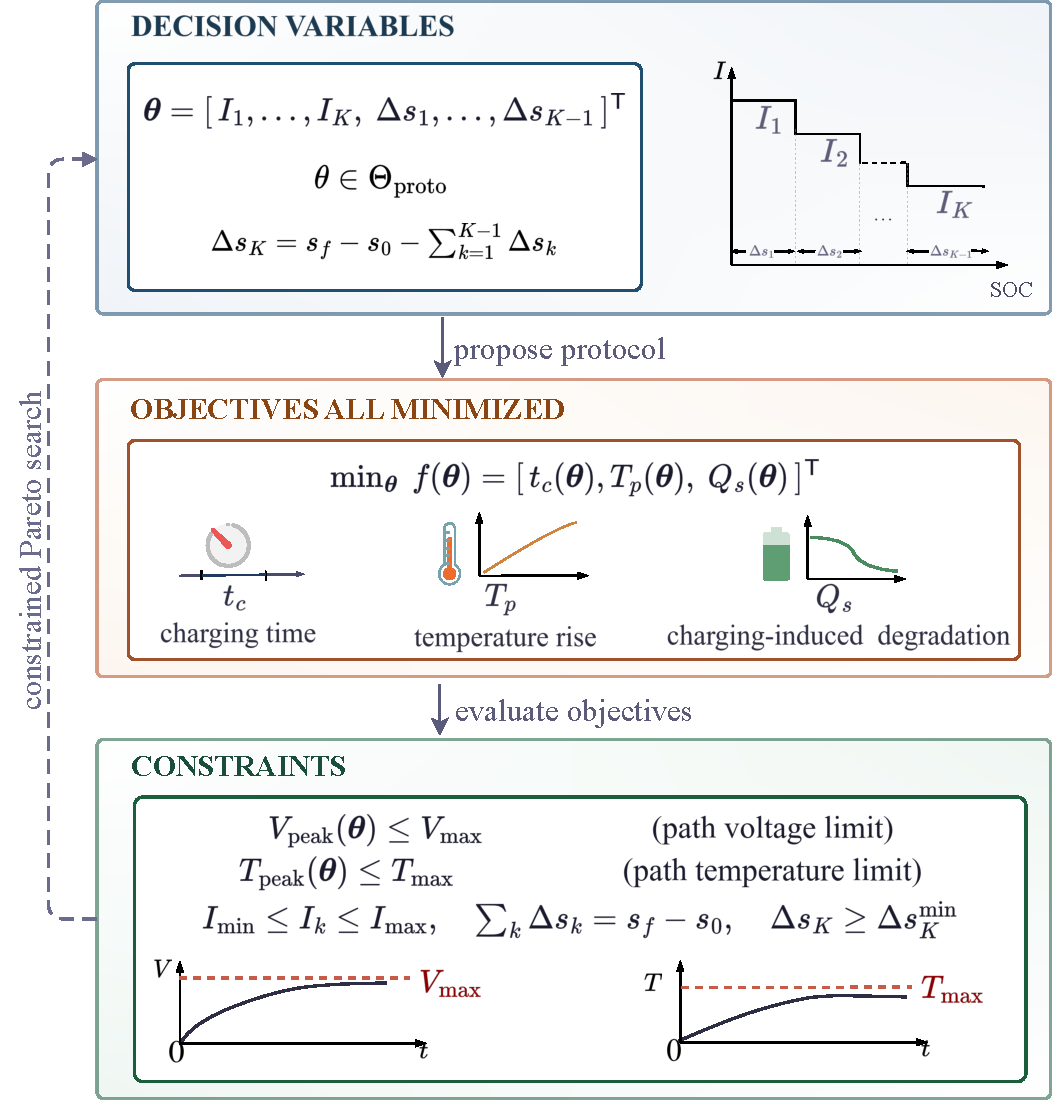
\includegraphics[width=\columnwidth]{fig1.pdf}
\caption{Fast-charging multiobjective design problem.}
\label{fig:charging_problem}
\end{figure}
% END: figures/fig_charging_design_problem.tex

\subsection{Multistage Constant-Current Protocol}

A $K$-stage protocol applies a current $I_k$ over an SOC increment $\Delta s_k$
at stage $k$, $k=1,\ldots,K$. The initial and target SOCs are $s_0$ and $s_f$,
respectively.
The independent decision variables are
\begin{equation}
\theta=[I_1,\ldots,I_K,\Delta s_1,\ldots,\Delta s_{K-1}]^\top
\label{eq:protocol}
\end{equation}
and the final SOC increment is
\begin{equation}
\Delta s_K=s_f-s_0-\sum_{k=1}^{K-1}\Delta s_k.
\label{eq:terminal_soc}
\end{equation}
Each current and SOC increment is restricted to its prescribed interval. The
last increment must also exceed a positive lower bound so that every stage has
nonzero duration.
% AUTHOR_CHECK P1: Supply the actual current/SOC bounds, terminal lower bound,
% initial and target SOCs, and effective capacities from the experiment configs.

Following~\cite{nref7,nref8}, the optimization is performed over SOC
increments rather than stage durations. The current and charge delivered in
each stage determine its duration, giving the total charging time
\begin{equation}
t_c(\theta)=3600Q_{\mathrm{eff}}\sum_{k=1}^{K}\frac{\Delta s_k}{I_k}
\label{eq:charging_time}
\end{equation}
where $Q_{\mathrm{eff}}$ is the effective cell capacity in Ah and current is
measured in A. The experiments use $K=3$, giving five independent decision
variables.

\subsection{Constrained Multiobjective Charging Design}

The three objectives are minimized jointly
\begin{equation}
\min_{\theta}\quad
\boldsymbol{f}(\theta)=[t_c(\theta),\,T_p(\theta),\,Q_s(\theta)]^\top.
\label{eq:cmop}
\end{equation}
Here, $T_p$ is the peak temperature rise and $Q_s$ is the aging indicator
defined in Section~\ref{sec:model_section}. In addition to the bounds on the
decision variables, the charging trajectory must satisfy
\begin{equation}
U(t;\theta)\le U_{\max},\quad
T(t;\theta)\le T_{\max},\quad
0\le t\le t_c(\theta)
\label{eq:operating_constraints}
\end{equation}
where $U(t;\theta)$ and $T(t;\theta)$ denote the terminal voltage and cell
temperature under protocol $\theta$, and $U_{\max}$ and $T_{\max}$ are the
corresponding voltage and temperature limits. A
protocol is infeasible if it violates either limit or fails to reach $s_f$;
such protocols are excluded from the Pareto set.
% AUTHOR_CHECK P2: Exclusion from the Pareto set does not specify how
% infeasible/failed simulations are represented in the GP or acquisition.

Higher charging currents reduce charging time but generally increase the
thermal and aging costs. A set of feasible nondominated protocols is
therefore sought, allowing the charging-time, temperature, and degradation trade-off
to be chosen for the operating requirement.
% END: sections/problem.tex
% Queue method illustrations early enough for the following page tops.
% BEGIN: figures/fig_llambo_mo_framework.tex
\begin{figure}[t]
\centering
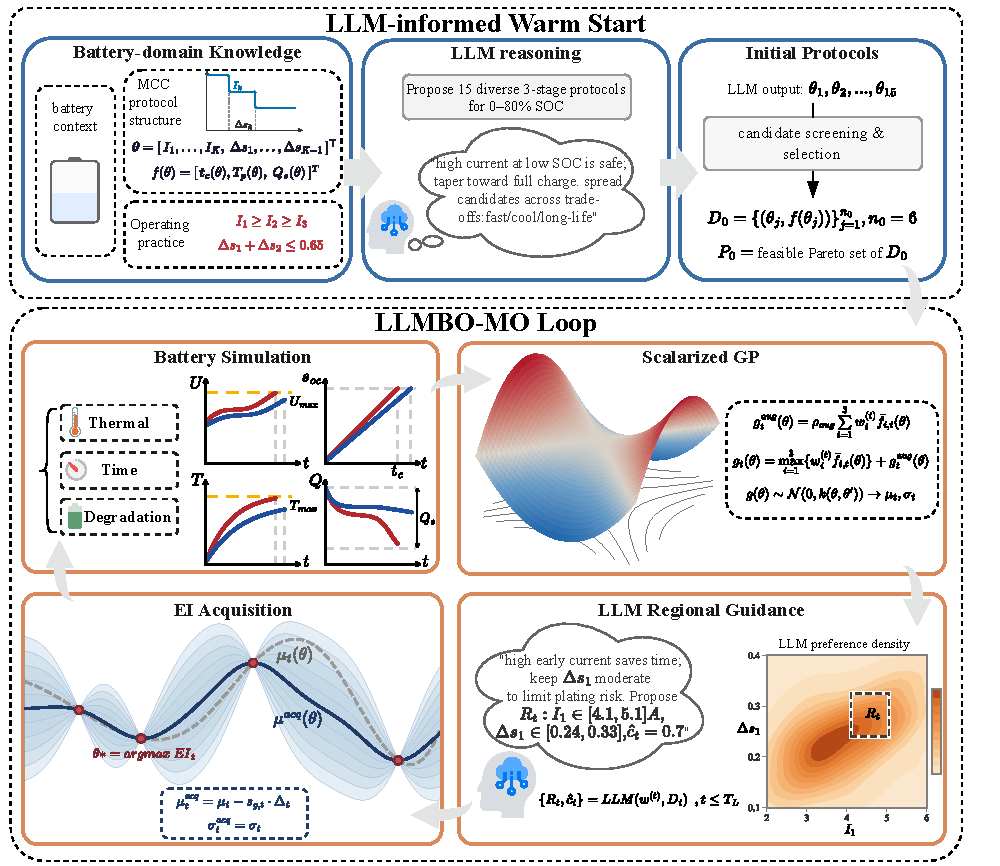
\includegraphics[width=\columnwidth]{fig2.pdf}
\caption{Structure of the proposed LLMBO-MO framework}
\label{fig:framework}
\end{figure}
% END: figures/fig_llambo_mo_framework.tex
% BEGIN: figures/fig_llm_prompts.tex
% Warm-start and regional prompts, paired side by side at the page top.
% Typeset in the style of boxed prompt figures: gray panel, thin frame,
% domain-knowledge phrases highlighted in red.
\newcommand{\promptbox}[1]{%
  \fcolorbox{black}{gray!10}{\parbox{\dimexpr\linewidth-2\fboxsep-2\fboxrule\relax}{#1}}}

% Paired figures share a page-top row so neither is stacked mid-column.
\begin{figure*}[t]
\centering
\begin{minipage}[t]{0.48\textwidth}
\vspace{0pt}
\centering
\promptbox{\footnotesize
You are an expert in \textcolor{red}{lithium-ion battery fast-charging
optimization}. Cell: LG INR21700-M50 (5~Ah, NMC811/graphite); the charging
window is 0\% to 80\% SOC.\\
Decision variables and bounds: $I_1\in[2.0,6.0]$~A,
$I_2\in[2.0,5.0]$~A, $I_3\in[2.0,3.0]$~A,
$\Delta s_1\in[0.10,0.40]$, $\Delta s_2\in[0.10,0.30]$.\\
Constraints: keep $\Delta s_1+\Delta s_2\le 0.65$ whenever possible
(practical hard limit $0.70$).
\textcolor{red}{A decreasing current profile $I_1\ge I_2\ge I_3$ is
recommended, since high currents at low SOC carry a lower risk of lithium
plating than the same currents near full charge.}\\
Objectives: minimize charging time, peak temperature rise, and capacity
fade.\\
Generate $15$ \textcolor{red}{diverse} protocols that
\textcolor{red}{cover multiple trade-off directions instead of clustering
around one style}. Respond with only a JSON array.}
\caption{Prompt for the LLM-informed warm start.}
\label{fig:prompt_warmstart}
\end{minipage}\hfill
\begin{minipage}[t]{0.48\textwidth}
\vspace{0pt}
% BEGIN: figures/fig_llm_region_prompt.tex
% Right-hand panel of the paired page-top prompt figures.
\centering
\promptbox{\footnotesize
You are guiding a battery charging Bayesian optimization loop.\\
Iteration $t$ of $T$; weight vector
$\mathbf w^{(t)}=(w_1,w_2,w_3)$; current best scalarized value
$g_t^{\mathrm{best}}$. Decision variables and bounds as in
Fig.~\ref{fig:prompt_warmstart}; hard constraint
$\Delta s_1+\Delta s_2<0.70$.\\
Return exactly one JSON object with one of two structures:\\
\hspace*{1em}\texttt{"point"}: \texttt{\{I1, I2, I3, dSOC1, dSOC2,
confidence\}}\\
\hspace*{1em}\texttt{"region"}: \texttt{\{lb: \{...\}, ub: \{...\},
confidence\}}\\
Guidelines: \textcolor{red}{use a point when confident about a specific
location; use a region when the promising area is uncertain} (region width
$5$--$20\%$ of the range per dimension). The confidence lies in $[0,1]$ and
\textcolor{red}{reflects your certainty}. All values must respect the
parameter bounds and the $\Delta s$ constraint. Output JSON only.}
\caption{Prompt for iteration-level regional guidance.}
\label{fig:prompt_region}
% END: figures/fig_llm_region_prompt.tex
\end{minipage}
\end{figure*}
% END: figures/fig_llm_prompts.tex
% BEGIN: sections/model.tex
\section{Electrochemical--Thermal--Aging Model}
\label{sec:model_section}

\subsection{Electrochemical Model}
\label{sec:model}

The single particle model with electrolyte dynamics (SPMe) describes the
battery's electrochemical response~\cite{refSPMe}. It accounts for lithium
diffusion in representative solid particles of both electrodes and transport
through the electrolyte. This reduced-order model retains the electrochemical
dynamics needed for charging simulation at a lower computational cost than a
full porous-electrode model.

The terminal voltage is calculated as~\cite{refSPMe}
\begin{equation}
U=U_{\mathrm{eq}}+\eta_r+\eta_d+\Delta\Phi
\label{eq:voltage}
\end{equation}
where $U_{\mathrm{eq}}$ is the equilibrium potential, $\eta_r$ is the ohmic
overpotential, $\eta_d$ is the concentration overpotential, and $\Delta\Phi$
is the average potential difference in the electrolyte. SOC is obtained from
the solid-phase lithium concentration. The SPMe equations and their derivation
are given in~\cite{refSPMe}.
% AUTHOR_CHECK M1: Verify the voltage decomposition and the meanings/signs of
% eta_r, eta_d, and DeltaPhi against the model actually implemented.

\subsection{Thermal Model}

A lumped thermal model gives the cell temperature
\begin{equation}
\rho_{\mathrm{eff}}\frac{\mathrm{d}T}{\mathrm{d}t}=\bar Q-\frac{hA}{V}(T-T_a).
\label{eq:thermal_balance}
\end{equation}
Here, $\rho_{\mathrm{eff}}$ is the effective volumetric heat capacity,
$\bar Q$ is the average volumetric heat-generation rate, $h$ is the
heat-transfer coefficient, $A$ is the heat-dissipation area, $V$ is the cell
volume, and $T_a$ is the ambient temperature. The effective heat capacity is
\begin{equation}
\rho_{\mathrm{eff}}=\frac{\sum_k\rho_kC_{p,k}L_k}{\sum_kL_k}
\label{eq:rho_eff}
\end{equation}
where $\rho_k$, $C_{p,k}$, and $L_k$ denote the density, specific heat
capacity, and thickness of layer $k$, and the sum runs over the five cell
layers, i.e., the two current collectors, the two electrodes, and the
separator.

The thermal objective is the maximum temperature rise during charging
\begin{equation}
T_p(\theta)=\max_{0\le t\le t_c(\theta)}[T(t)-T_0]
\label{eq:peak_temp}
\end{equation}
where $T_0$ is the initial cell temperature.

\subsection{Aging Model}
\label{sec:aging}

Charging-induced degradation is evaluated with the semi-empirical
capacity-loss model of Suri and Onori~\cite{refAgingModel}
\begin{equation}
Q_s(\xi,Ah)=\sigma_{\mathrm{fun}}(\xi)Ah^z.
\label{eq:aging}
\end{equation}
The vector $\xi=(\mathrm{SOC},I,T)$ contains the average SOC, current, and
temperature during charging; $Ah$ is the charge throughput; and $z$ is the
power-law exponent. The severity factor is
% AUTHOR_CHECK M2: The uploaded equation is preserved below. Its denominator
% uses 273.15+T, whereas the thermal settings use kelvin. Verify the conversion
% in the implementation before choosing a Celsius or kelvin notation here.
\begin{equation}
\sigma_{\mathrm{fun}}(\xi)=(\alpha\,\mathrm{SOC}+\beta)\exp\!\left(\frac{-E_a+\eta_a I}{R_{\mathrm{gas}}(273.15+T)}\right)
\label{eq:severity}
\end{equation}
where $\alpha$ and $\beta$ describe SOC dependence, $\eta_a$ describes current
dependence, $E_a$ is the activation energy, and $R_{\mathrm{gas}}$ is the
universal gas constant. In (4), $Q_s(\theta)$ denotes $Q_s(\xi,Ah)$
evaluated with the charging-averaged quantities $\xi$ and the charge
throughput $Ah$ induced by protocol $\theta$. It serves as a relative
degradation indicator for one charging process, rather than as a prediction
of battery end-of-life.
% AUTHOR_CHECK M3: Supply the coefficients, averaging/aggregation rule, and
% justification for using this aging model with each battery parameterization.
% END: sections/model.tex
% BEGIN: sections/method.tex
% ============================================================================
% Section IV: Proposed LLMBO-MO
% Revised to emphasize the core methodological idea and reduce implementation-level detail.
% ============================================================================

\section{Proposed LLMBO-MO}
\label{sec:method}

\subsection{Framework}
\label{sec:framework}

LLMBO-MO uses battery-domain knowledge to guide the choice of protocols to
simulate. The optimization loop is shown in Fig.~\ref{fig:framework}. The LLM
first proposes an initial set of protocols. During the early BO iterations,
it also suggests a region for the current trade-off among objectives. The BO
optimizer scalarizes the observed objectives, fits a GP, and selects the next
protocol by maximizing EI. Evaluating that protocol with the battery model
provides its objective values and feasibility, which are used to update the
data set $D$ and the feasible Pareto set $P$. The loop stops when the
simulation budget is exhausted.

\subsection{Decomposition-Based Multiobjective BO}
\label{sec:parego_backbone}

The numerical optimizer follows the decomposition-based approach of
EIMO~\cite{refEIMO}. A set $W$ of nonnegative weight vectors represents
trade-offs among the three objectives. At iteration $t$, the optimizer selects
$\mathbf w^{(t)}=[w_1^{(t)},w_2^{(t)},w_3^{(t)}]$ from $W$, with
$\sum_{i=1}^{3}w_i^{(t)}=1$.

Charging time and aging are first transformed to reduce differences in scale
\begin{equation}
 y_1(\theta)=\log\!\frac{t_c(\theta)}{t_{\mathrm{ref}}},
 y_2(\theta)=T_p(\theta),
 y_3(\theta)=\log\!\frac{Q_s(\theta)}{Q_{\mathrm{ref}}}
 \label{eq:objective_transform}
\end{equation}
where $t_{\mathrm{ref}}$ and $Q_{\mathrm{ref}}$ are fixed positive reference
values. A positive floor is applied before taking logarithms. Let
$z_{i,t}^{*}$ be the best observed value of transformed objective $i$ and
$s_{i,t}$ its scaling factor. The normalized distance is
\begin{equation}
 \bar f_{i,t}(\theta)=
 \frac{|y_i(\theta)-z_{i,t}^{*}|}{s_{i,t}},\qquad i=1,2,3.
 \label{eq:objective_scaling}
\end{equation}
The augmented Tchebycheff scalarization combines these distances
\begin{equation}
 g_t(\theta)=
 \max_{i=1,2,3}\!\left\{w_i^{(t)}\bar f_{i,t}(\theta)\right\}
 +\rho_{\mathrm{aug}}\sum_{i=1}^{3}w_i^{(t)}\bar f_{i,t}(\theta)
 \label{eq:tchebycheff}
\end{equation}
where $\rho_{\mathrm{aug}}>0$ is a small augmentation coefficient. Changing
$\mathbf w^{(t)}$ directs successive iterations toward different parts of the
Pareto front.

A GP with an automatic relevance determination (ARD) Mat\'ern-$5/2$ kernel is
fitted to the scalarized observations. Its posterior mean and standard
deviation are denoted by $\mu_t(\theta)$ and $\sigma_t(\theta)$. For
minimization, EI is
\begin{align}
 x_t&=\frac{g_t^{\mathrm{best}}-\mu_t(\theta)}{\sigma_t(\theta)}\\
 \mathrm{EI}_t(\theta)
 &=\bigl(g_t^{\mathrm{best}}-\mu_t(\theta)\bigr)\Phi(x_t)
 +\sigma_t(\theta)\phi(x_t)
 \label{eq:ei}
\end{align}
where $g_t^{\mathrm{best}}$ is the best observed scalarized value, and
$\Phi$ and $\phi$ are the standard normal cumulative distribution and density
functions.

\subsection{LLM-Informed Warm Start}
\label{sec:warm_start}

The first GP is fitted to a small initial data set. To make these evaluations
more informative for charging design, the LLM is given the battery context,
MCC protocol structure, decision-variable bounds, objectives, and domain
knowledge about charging (Fig.~\ref{fig:prompt_warmstart}). It returns
numerical candidate protocols and a preference ranking.

The candidate pool is screened before simulation. Entries with non-numerical
or non-finite values, duplicates, and invalid protocol representations are
removed; out-of-bound values are repaired. The remaining candidates are
selected using their ranking and diversity in the decision space. Random
valid protocols supplement this selection to cover other parts of the search
space. The resulting $n_0$ protocols are simulated to initialize the data
set and the Pareto set.

\subsection{Regional Guidance}
\label{sec:region_pref}

The warm start introduces LLM suggestions before sequential
optimization begins. During the search, the relevant trade-off changes with
the scalarization weights. At an early iteration $t$, the LLM therefore receives the current
weights $\mathbf w^{(t)}$ and the observed optimization state, and returns a
preferred region $R_t$ for that subproblem
(Fig.~\ref{fig:prompt_region}). Restricting the search to $R_t$
would exclude all candidates outside the proposed region. Instead, the regional
guidance uses GP posterior cross-covariance to adjust their acquisition values. This
extends LGBO's region-lifted preference mechanism~\cite{ref5} to the current
scalarized objective.

A valid region is represented by $M$ Sobol anchors
$G_t=\{\mathbf g_{1,t},\ldots,\mathbf g_{M,t}\}$ with equal weights
$\mathbf v_t=(1/M)\mathbf 1$, where $M$ is the number of anchors and
$\mathbf 1$ is the $M$-dimensional all-ones vector. Let
$\widetilde{\boldsymbol\Sigma}_{GG,t}$ and
$\widetilde{\boldsymbol\Sigma}_{\theta G,t}$ denote the posterior covariance
matrix of the scalarized GP at the anchors and the posterior cross-covariance
between a candidate $\theta$ and the anchors, respectively. The average of
the GP function values at these anchors has posterior variance
\begin{equation}
 V_{G,t}=\mathbf v_t^{\top}
 \widetilde{\boldsymbol\Sigma}_{GG,t}\mathbf v_t.
 \label{eq:region_variance}
\end{equation}
The covariance between the candidate value and this regional average is
$\widetilde{\boldsymbol\Sigma}_{\theta G,t}\mathbf v_t$. It determines the
candidate's adjustment
\begin{equation}
 r_t(\theta)=
 \lambda_t\,
 \frac{\widetilde{\boldsymbol\Sigma}_{\theta G,t}\mathbf v_t}
 {\sqrt{V_{G,t}}},
 \quad
 \lambda_t\propto
 \widehat c_t\max\!\left(1-\frac{t-1}{T_{\mathrm L}},0\right).
 \label{eq:region_adjustment}
\end{equation}
Here, $\widehat c_t$ is the guidance score returned by the LLM, and
$T_{\mathrm L}$ is the guidance horizon. The coefficient $\lambda_t$ combines
this score with a fixed scale and a linearly decaying time factor. Positive posterior
cross-covariance produces a favorable adjustment for the minimization
problem; negative cross-covariance produces the opposite adjustment.

The adjustment $r_t(\theta)$ is rescaled using its magnitude at the regional
anchors and clipped to obtain a bounded value $\Delta_t(\theta)$. If
$s_{g,t}$ is the scale of the scalar GP target, EI is computed using
\begin{equation}
 \mu_t^{\mathrm{acq}}(\theta)
 =\mu_t(\theta)-s_{g,t}\Delta_t(\theta),
 \quad
 \sigma_t^{\mathrm{acq}}(\theta)=\sigma_t(\theta).
 \label{eq:region_acq_mean}
\end{equation}
Thus, a positive adjustment lowers the mean used by EI while leaving the
fitted GP and its posterior variance unchanged. Standard EI is used when no
valid region is available and after the guidance window.
The overall procedure is summarized in Algorithm~\ref{alg:llmbo}.

\begin{algorithm}[t]
\caption{LLMBO-MO}
\label{alg:llmbo}
\footnotesize
\begin{algorithmic}[1]
\Require Battery simulator, LLM, total budget $N$, initial budget $n_0$, weight set $W$, guidance horizon $T_{\mathrm L}$
\Ensure Feasible Pareto set $P$
\State Generate and screen LLM-informed warm-start protocols
\State Combine selected LLM proposals with random valid protocols
\State Evaluate the $n_0$ initial protocols; initialize $D$ and $P$
\For{$t=1$ to $N-n_0$}
    \State Select $\mathbf w^{(t)}\in W$ and compute $g_t$ using Eq.~\eqref{eq:tchebycheff}
    \State Fit the scalar GP and construct EI
    \If{$t\le T_{\mathrm L}$}
        \State Query the LLM for a preferred region under $\mathbf w^{(t)}$
        \If{a valid region is returned}
            \State Apply regional guidance using Eqs.~\eqref{eq:region_variance}--\eqref{eq:region_acq_mean}
        \EndIf
    \EndIf
    \State Maximize EI and select the next protocol $\theta_{t+1}$
    \State Evaluate $\theta_{t+1}$ and append the result to $D$
    \State Update the feasible Pareto set $P$
\EndFor
\State \Return $P$
\end{algorithmic}
\end{algorithm}
% END: sections/method.tex
% BEGIN: sections/experiments.tex
\section{Numerical Validation and Discussion}
\label{sec:experiments}

The experiments examine whether LLM guidance improves charging optimization
at a fixed simulation budget and which part of the guidance accounts for the
gain. Comparisons with other optimizers are followed by initialization and
component studies. LLM backends are also compared, and representative
charging protocols from the computed Pareto set are inspected.

\begin{table}[!t]
\caption{Battery and Simulator Settings}
\label{tab:battery_settings}
\centering
\footnotesize
\setlength{\tabcolsep}{3.0pt}
\begin{tabular}{@{}>{\raggedright\arraybackslash}p{0.58\columnwidth}
                    >{\raggedright\arraybackslash}p{0.34\columnwidth}@{}}
\toprule
Parameter & Value \\
\midrule
Primary parameterization & Chen2020, LG INR21700-M50 \\
Additional parameterization & Ecker2015 \\
Chen2020 nominal capacity & 5.0 Ah \\
Chen2020 cell voltage range & 2.50--4.20 V \\
Chen2020 cell format & 21700 cylindrical, 70 $\times$ 21 mm \\
Initial/ambient temperature & 298.15 K \\
Maximum cell temperature & 328.15 K \\
Total heat transfer coefficient & 17.36 W\,m$^{-2}$\,K$^{-1}$ \\
Negative electrode diffusivity & $3.96\times10^{-14}$ m$^2$\,s$^{-1}$ \\
Positive electrode diffusivity & $4.80\times10^{-15}$ m$^2$\,s$^{-1}$ \\
\bottomrule
\end{tabular}
\end{table}

\begin{table}[!t]
\caption{Main Experimental Settings}
\label{tab:algorithm_settings}
\centering
\footnotesize
\setlength{\tabcolsep}{3.0pt}
\begin{tabular}{@{}>{\raggedright\arraybackslash}p{0.62\columnwidth}
                    >{\raggedright\arraybackslash}p{0.30\columnwidth}@{}}
\toprule
Setting & Value \\
\midrule
Total simulator budget & 56 \\
Initial evaluations & 6 \\
Number of matched trials & 5 \\
Initial LLM candidate pool & 15 \\
Region-guided horizon $T_{\mathrm L}$ & \RegionHorizon \\
Number of regional anchors $M$ & \RegionAnchors \\
Tchebycheff coefficient $\rho_{\mathrm{aug}}$ & \RhoAug \\
\bottomrule
\end{tabular}
\end{table}

\subsection{Experimental Setup}

The optimization environment is an electrochemical--thermal--aging model
developed in PyBaMM, with model parameters taken from experimentally
identified parameterizations of real lithium-ion cells. The main case uses
the Chen2020 parameterization of the LG INR21700-M50
cell~\cite{ref8}. A second case uses Ecker2015~\cite{ref9} to examine
performance with a different battery parameterization. The objectives are
charging time $t_c$, peak temperature rise $T_p$, and aging indicator $Q_s$.
The battery and algorithm settings are summarized in
Tables~\ref{tab:battery_settings} and~\ref{tab:algorithm_settings}.

The main comparison allocates 56 battery-model evaluations to each method
and uses five matched trials. For the BO methods, this budget consists of six
initial evaluations and 50 subsequent iterations. Hypervolume (HV) measures
the quality of the feasible nondominated set; larger values are better under
the same objective definitions and reference point. All methods use the same
HV calculation within each battery parameterization. Final HV is reported as
mean $\pm$ sample standard deviation.

ParEGO is the primary BO baseline because it uses the same decomposition--GP
structure as the numerical optimizer in LLMBO-MO~\cite{ref4}. DISK and PIMD
provide comparisons with surrogate-assisted multiobjective
evolutionary optimization~\cite{refDISK,refPIMD}; NSGA-II is included as a
classical evolutionary baseline~\cite{refNSGAII}.

% Paired figures share a page-top row so neither is stacked mid-column.
\begin{figure*}[t]
\centering
\begin{minipage}[t]{0.48\textwidth}
\vspace{0pt}
\centering
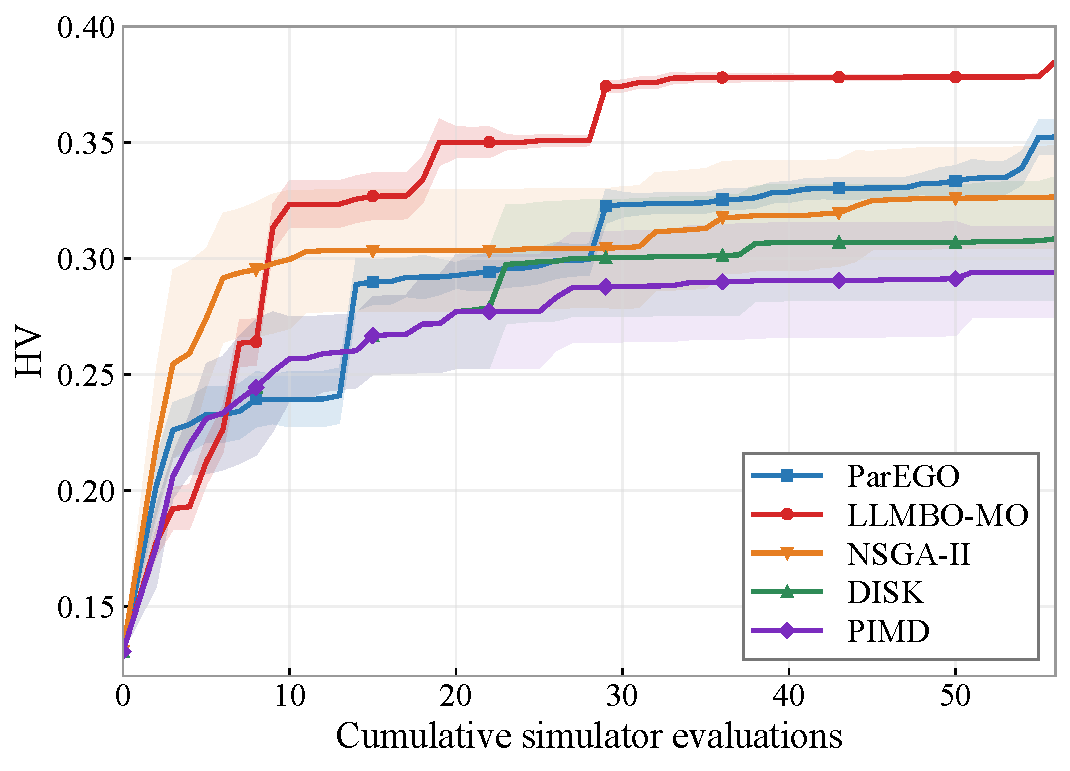
\includegraphics[width=0.99\linewidth]{chen2020_hv_5way.pdf}
\caption{HV trajectories of the five methods on Chen2020.}
\label{fig:chen_hv_5way}
\end{minipage}\hfill
\begin{minipage}[t]{0.48\textwidth}
\vspace{0pt}
\centering
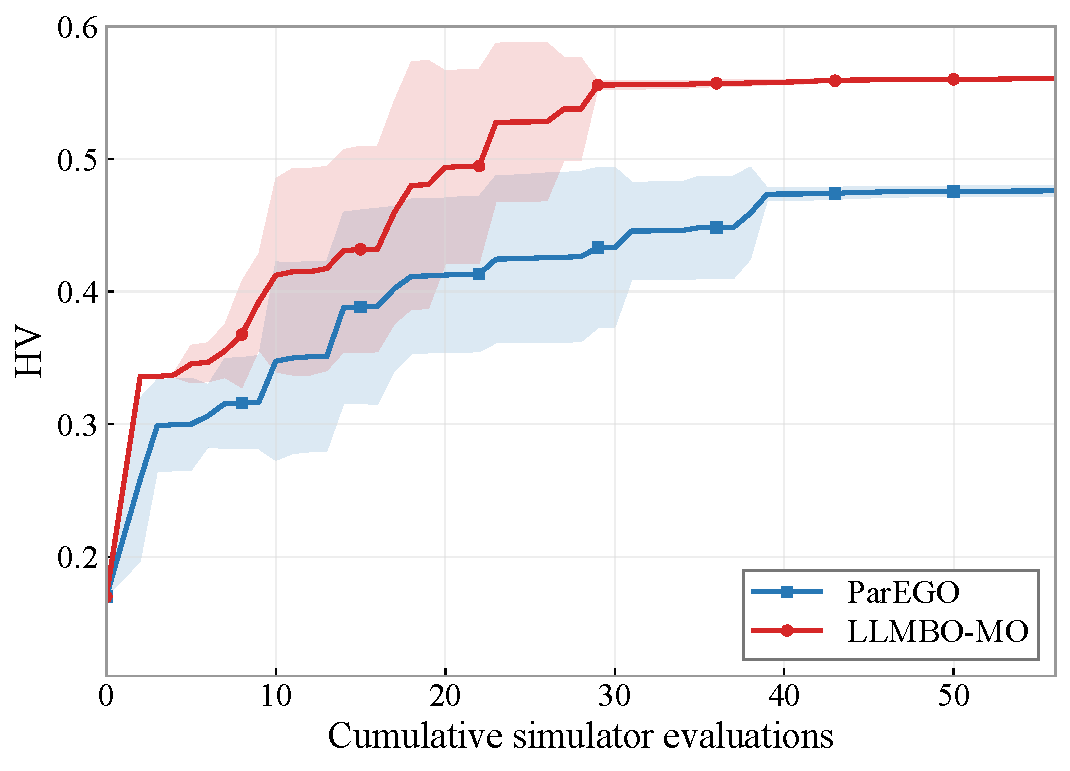
\includegraphics[width=0.99\linewidth]{ecker2015_hv.pdf}
\caption{HV trajectories of LLMBO-MO and ParEGO on Ecker2015.}
\label{fig:ecker_hv}
\end{minipage}
\end{figure*}

\begin{table}[!t]
\caption{Final HV on Chen2020}
\label{tab:chen_results}
\centering
\footnotesize
\setlength{\tabcolsep}{4.0pt}
\begin{tabular}{@{}lc@{}}
\toprule
Method & Final HV (mean $\pm$ SD) $\uparrow$ \\
\midrule
LLMBO-MO & \textbf{\ChenLLMBOMean\,$\pm$\,\ChenLLMBOStd} \\
ParEGO & \ChenParEGOMean\,$\pm$\,\ChenParEGOStd \\
NSGA-II & \ChenNSGAMean\,$\pm$\,\ChenNSGAStd \\
DISK & \ChenDISKMean\,$\pm$\,\ChenDISKStd \\
PIMD & \ChenPIMDMean\,$\pm$\,\ChenPIMDStd \\
\bottomrule
\end{tabular}
\end{table}

\subsection{Performance Comparison}

LLMBO-MO obtains the highest final mean HV among the five methods on Chen2020
(Table~\ref{tab:chen_results}). After 56 evaluations, its mean HV is
\ChenLLMBOMean\,$\pm$\,\ChenLLMBOStd, compared with
\ChenParEGOMean\,$\pm$\,\ChenParEGOStd\ for ParEGO, a
\ChenFinalGain\ increase. NSGA-II, DISK, and PIMD reach mean HV values of
\ChenNSGAMean, \ChenDISKMean, and \ChenPIMDMean, respectively.
As shown in Fig.~\ref{fig:chen_hv_5way}, the lead over ParEGO develops early
in the search and persists to the end of the budget.

\begin{table}[!t]
\caption{HV Comparison on Ecker2015}
\label{tab:ecker_results}
\centering
\footnotesize
\setlength{\tabcolsep}{4.0pt}
\begin{tabular}{@{}lc@{}}
\toprule
Method & Evaluation 56 \\
\midrule
ParEGO & \EckerParEGOMean\,$\pm$\,\EckerParEGOStd \\
LLMBO-MO & \textbf{\EckerLLMBOMean\,$\pm$\,\EckerLLMBOStd} \\
\bottomrule
\end{tabular}
\end{table}

The comparison with ParEGO is repeated on Ecker2015. LLMBO-MO reaches
\EckerLLMBOMean\,$\pm$\,\EckerLLMBOStd\ at evaluation 56, whereas ParEGO
reaches \EckerParEGOMean\,$\pm$\,\EckerParEGOStd
(Table~\ref{tab:ecker_results}). Its HV is also higher over most of the search
in Fig.~\ref{fig:ecker_hv}. The advantage over ParEGO is therefore observed
with both battery parameterizations at the tested budget.

\subsection{Ablation Study}

The preceding comparisons assess the complete method. Two studies on
Chen2020 separate the effect of battery-specific prompting from the
contributions of the warm start and regional guidance.

% Paired figures share a page-top row so neither is stacked mid-column.
\begin{figure*}[t]
\centering
\begin{minipage}[t]{0.48\textwidth}
\vspace{0pt}
\centering
\promptbox{\footnotesize
You are an expert in lithium-ion battery fast-charging optimization. Task:
design $15$ diverse initial charging protocols for a multi-objective
Bayesian optimization workflow.\\
Decision variables and bounds: $I_1\in[2.0,6.0]$~A,
$I_2\in[2.0,5.0]$~A, $I_3\in[2.0,3.0]$~A,
$\Delta s_1\in[0.10,0.40]$, $\Delta s_2\in[0.10,0.30]$; hard constraint
$\Delta s_1+\Delta s_2<0.70$.\\
Objectives: minimize charging time, peak temperature rise, and capacity
fade.\\
Guidance: multi-objective optimization requires exploring different
trade-off directions (fast charging vs.\ thermal safety vs.\ aging
minimization); a good initial set should be well dispersed across the
five-dimensional decision space;
\textcolor{red!70!black}{consider leveraging physical relationships
between decision variables}; points near the boundary of the feasible
region can help maximize Pareto coverage, while interior points help model
the response surface in the central region. Respond with only a JSON
array.}
\caption{Generic prompt used in the initialization study of
Table~\ref{tab:prompt_study}. Unlike the battery-specific prompt in
Fig.~\ref{fig:prompt_warmstart}, it contains no battery-specific domain
knowledge.}
\label{fig:prompt_generic}
\end{minipage}\hfill
\begin{minipage}[t]{0.48\textwidth}
\vspace{0pt}
\centering

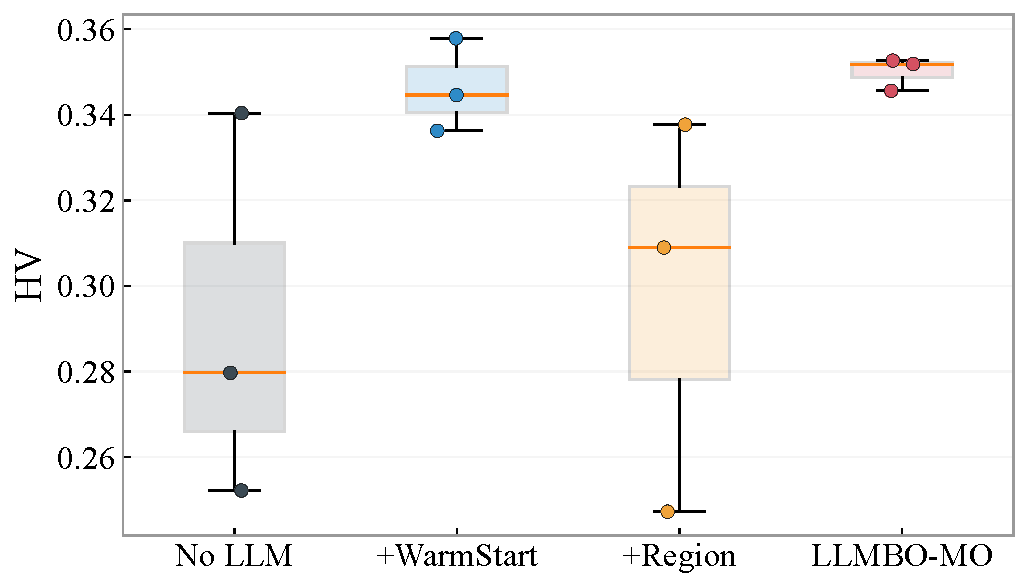
\includegraphics[width=0.99\linewidth]{ablation_hv_box.pdf}

\caption{Final HV distributions of the four ablation variants on Chen2020.}

\label{fig:ablation_hv_box}
\end{minipage}
\end{figure*}

% Paired figures share a page-top row so neither is stacked mid-column.
% Declared before the bibliography so the floats land on an earlier page.
\begin{figure*}[t]
\centering
\begin{minipage}[t]{0.48\textwidth}
\vspace{0pt}
\centering
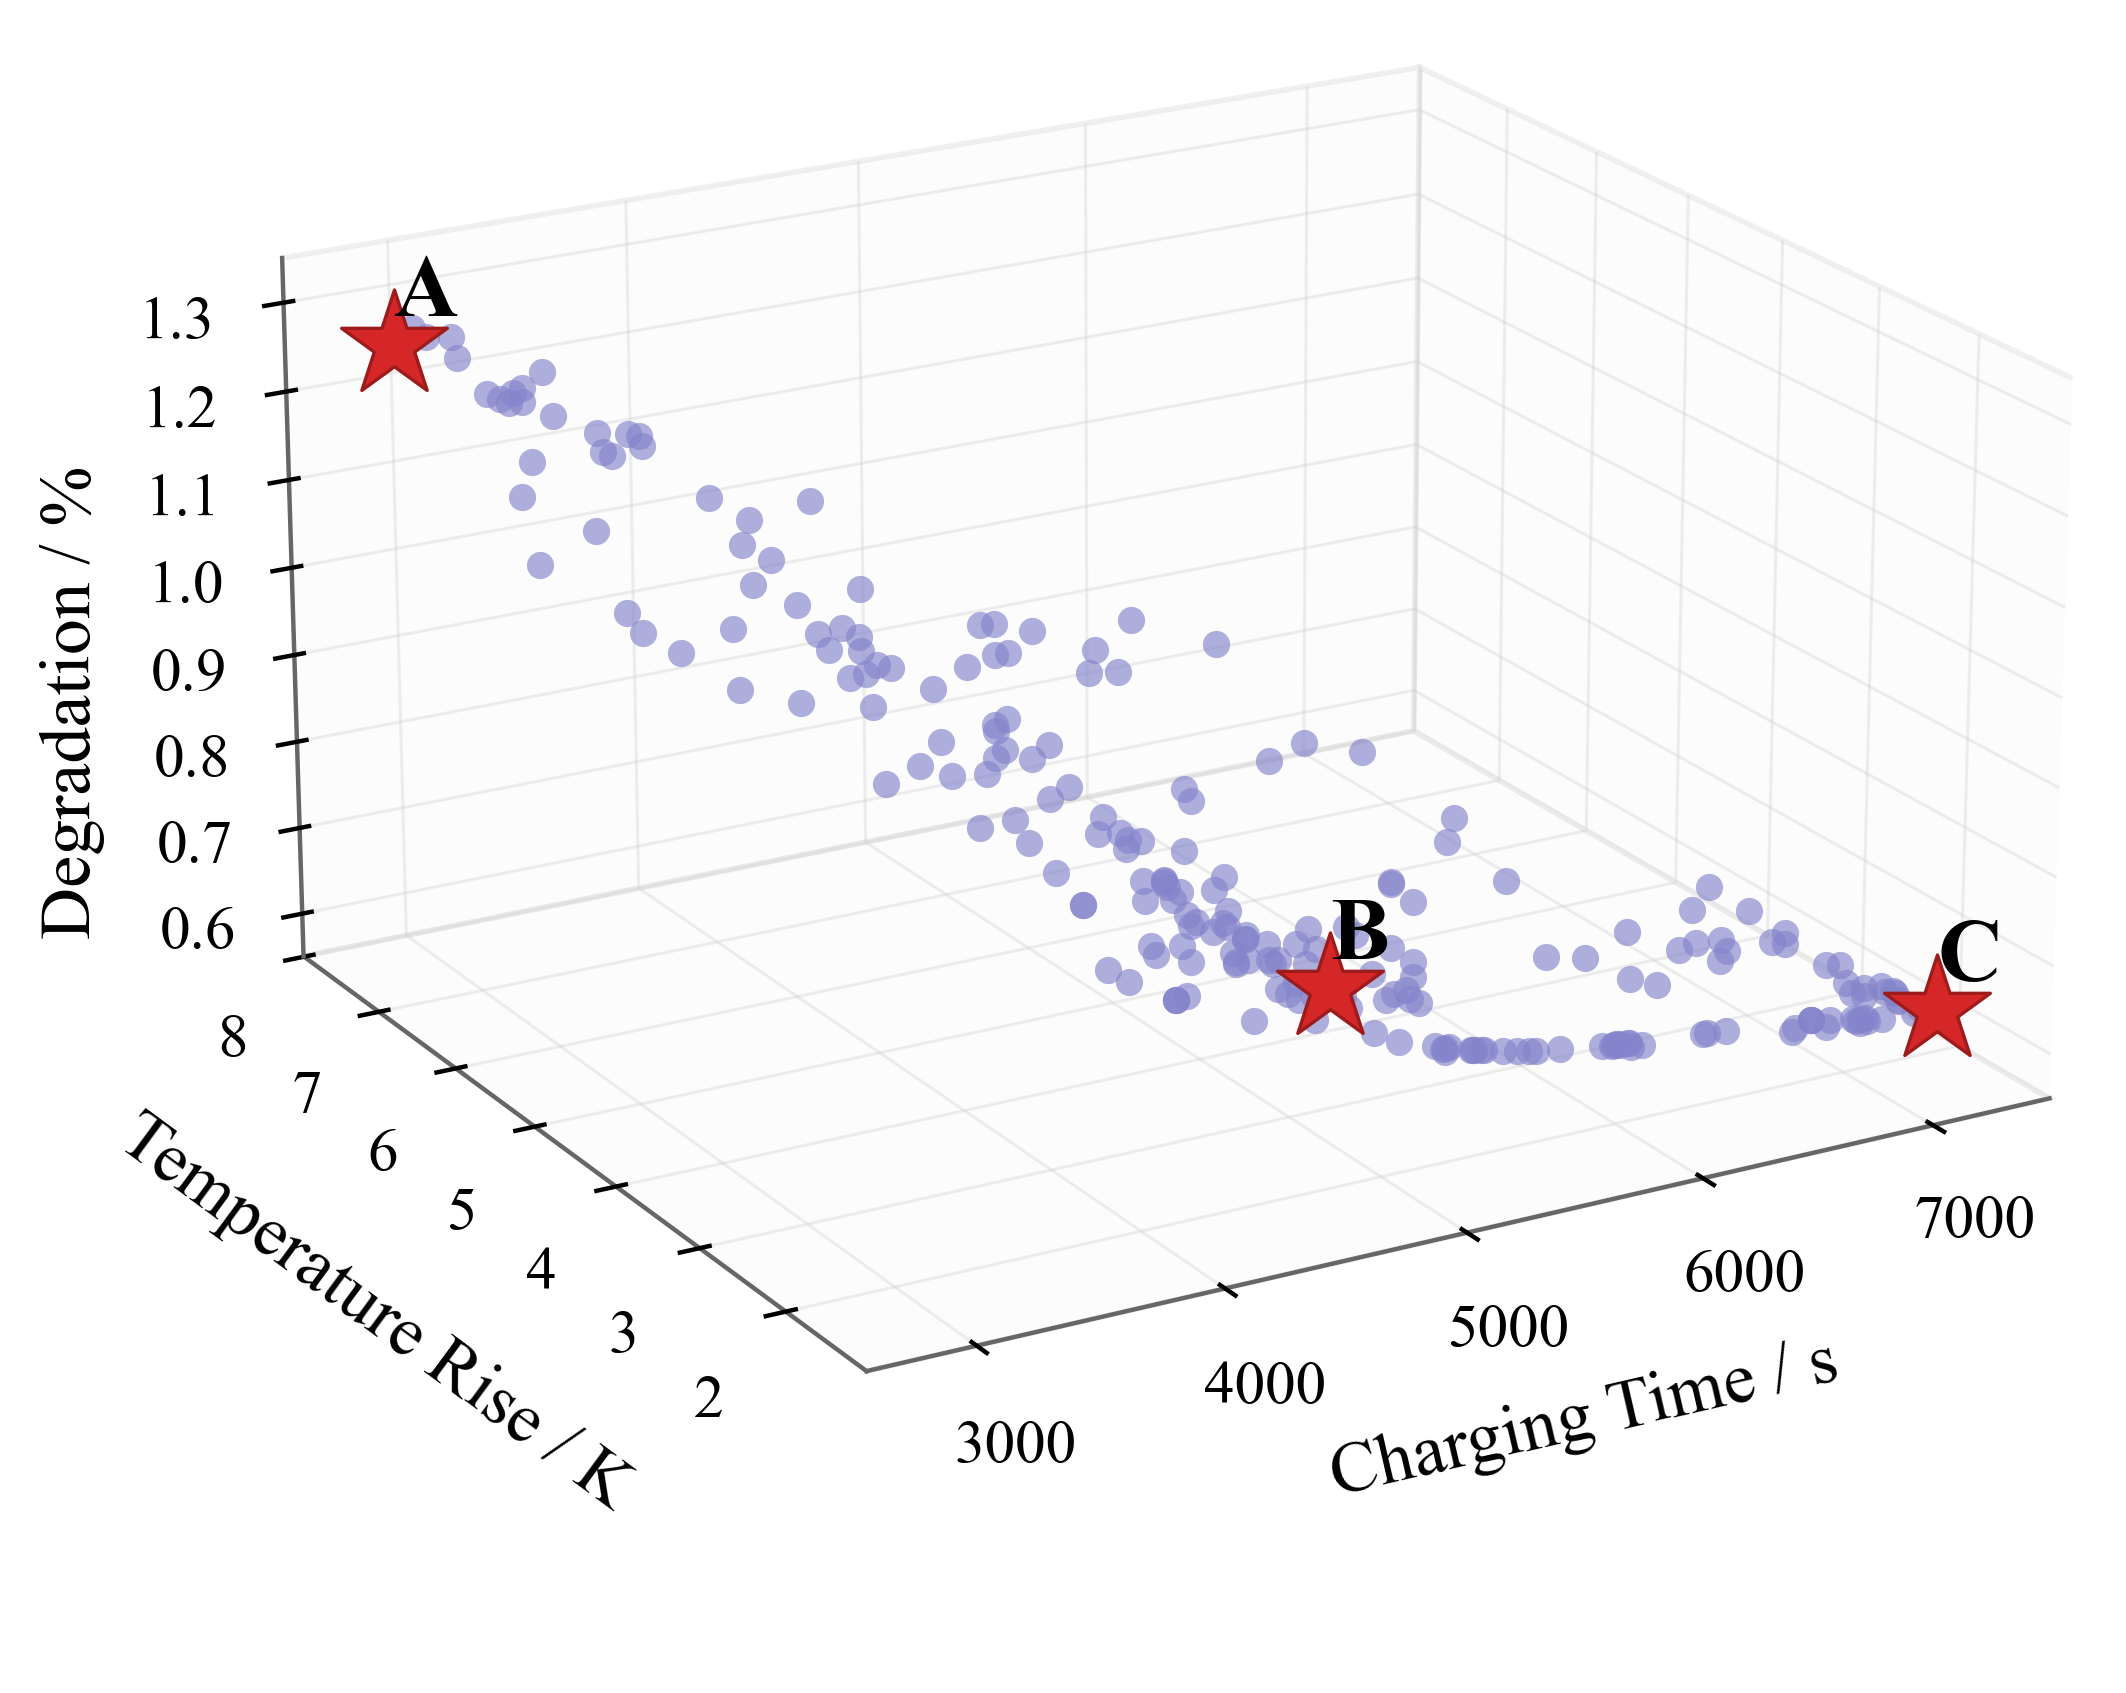
\includegraphics[width=\linewidth]{pareto_protocols_ae.png}
\caption{Representative charging protocols from the computed Pareto set on Chen2020.}
\label{fig:pareto_profiles}
\end{minipage}\hfill
\begin{minipage}[t]{0.48\textwidth}
\vspace{0pt}
\centering
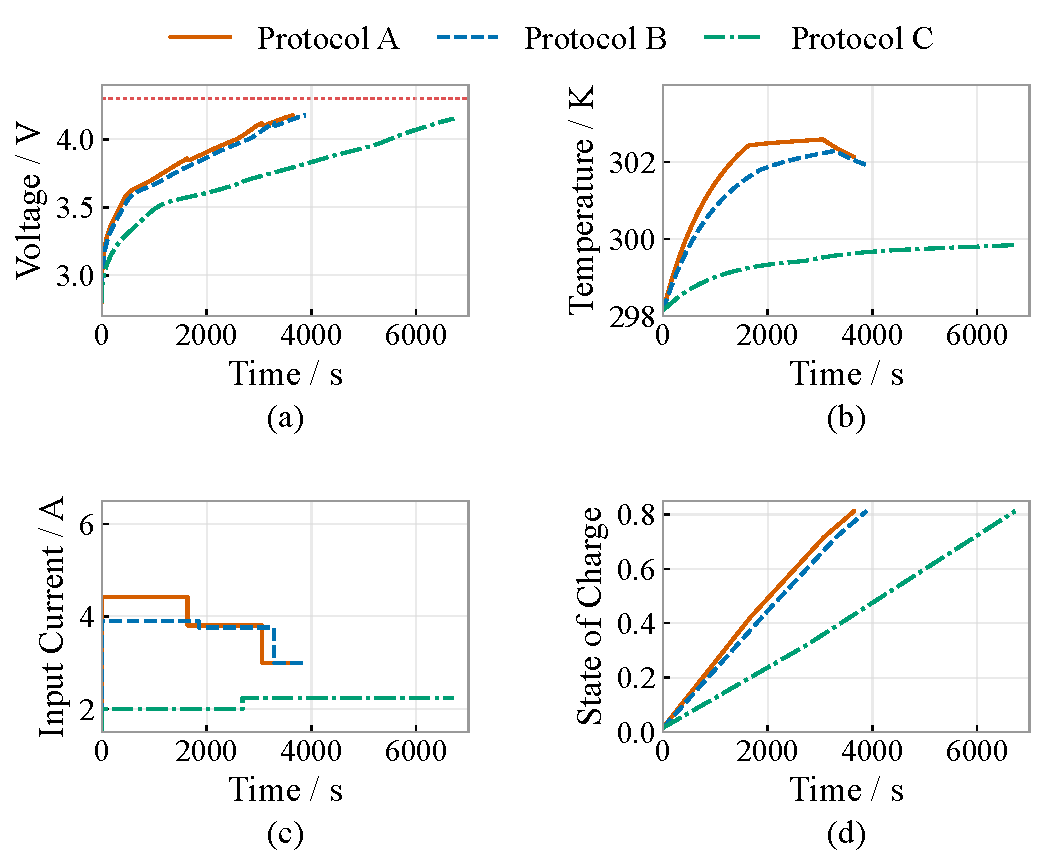
\includegraphics[width=\linewidth]{abc_charging_profiles.pdf}
\caption{Charging trajectories of protocols A--C on Chen2020.}
\label{fig:abc_charging_profiles}
\end{minipage}
\end{figure*}

\begin{table}[!t]
\caption{Effect of Different Initialization Strategies}
\label{tab:prompt_study}
\centering
\footnotesize
\setlength{\tabcolsep}{4.0pt}
\begin{tabular}{@{}lc@{}}
\toprule
Initialization & Final HV (mean $\pm$ SD) $\uparrow$ \\
\midrule
Random & 0.31062 $\pm$ 0.04303 \\
Generic prompt & 0.31371 $\pm$ 0.04675 \\
Battery-specific prompt & \textbf{0.36890 $\pm$ 0.00824} \\
\bottomrule
\end{tabular}
\end{table}

\subsubsection{LLM-Informed Warm Start}

Random initialization, a detailed generic prompt, and a
battery-specific prompt are compared (Figs.~\ref{fig:prompt_warmstart}
and~\ref{fig:prompt_generic}). All three variants use the same numerical BO
procedure after initialization. Each run has a budget of 26 evaluations,
and the results are computed over ten matched trials
(Table~\ref{tab:prompt_study}).

The generic prompt gives a mean final HV close to that of random
initialization: 0.31371 versus 0.31062. The battery-specific prompt reaches
0.36890, an increase of \PromptHVGain\ over random initialization, and has a
smaller standard deviation. The paired initialization analysis yields a
Holm-adjusted $p$-value of \PromptHolmP. The difference between generic and
battery-specific prompting indicates that the content of the domain
information matters for short-budget optimization, not merely the use of an
LLM to generate candidates.

\begin{table}[!t]

\caption{Ablation Results on Chen2020}

\label{tab:ablation}

\centering

\footnotesize

\setlength{\tabcolsep}{4.0pt}

\begin{tabular}{@{}lc@{}}

\toprule

Variant & Final HV (mean $\pm$ SD) $\uparrow$ \\

\midrule

No LLM & \AblationBaselineMean\,$\pm$\,\AblationBaselineStd \\

+ Warm start & \AblationWarmMean\,$\pm$\,\AblationWarmStd \\

+ Regional guidance & \AblationRegionMean\,$\pm$\,\AblationRegionStd \\

LLMBO-MO & \textbf{\AblationFullMean\,$\pm$\,\AblationFullStd} \\

\bottomrule

\end{tabular}

\end{table}

\subsubsection{Regional Guidance}

Four variants are compared: the numerical BO optimizer without LLM guidance,
warm start only, regional guidance only, and the complete method. This
study uses three matched trials per variant. Each run contains six initial
evaluations followed by 50 BO iterations, giving a total budget of 56
battery-model evaluations. The results are summarized in
Table~\ref{tab:ablation} and Fig.~\ref{fig:ablation_hv_box}.

As shown in Fig.~\ref{fig:ablation_hv_box} and Table~\ref{tab:ablation},
the LLM-informed warm start provides the largest improvement among the two
components. Adding the warm start increases the mean final HV from
\AblationBaselineMean\ to \AblationWarmMean, whereas regional guidance alone
reaches \AblationRegionMean. When regional guidance is added on top of the
warm start, the mean final HV further increases from
\AblationWarmMean\ to \AblationFullMean. The complete method also has the
smallest sample standard deviation among the four variants.

The results indicate that the two components contribute at different stages
of the optimization. The warm start improves the starting design
by directing the initial evaluations toward more promising charging protocols.
The regional guidance then uses the current scalarization weights to adjust
candidate selection during the subsequent BO iterations. In this comparison,
the warm start provides most of the performance gain, while regional guidance
further improves the final optimization result.

\begin{table}[!t]

\caption{HV Obtained with Different LLM Backends}

\label{tab:llm_backends}

\centering

\footnotesize

\setlength{\tabcolsep}{4.5pt}

\begin{tabular}{@{}lccc@{}}

\toprule

Backend & Initial HV & HV at 15 & Final HV \\

\midrule

DeepSeek-V4-Flash & 0.341225 & \textbf{0.373845} & 0.385986 \\

DeepSeek-V4-Pro & 0.345274 & 0.372526 & \textbf{0.387931} \\

GLM-5.3-Flash & \textbf{0.346248} & 0.372527 & 0.385324 \\

\bottomrule

\end{tabular}

\end{table}

\subsection{Comparison Across LLM Backends}

\label{sec:llm_backends}

To examine the effect of the LLM backend, three backends are compared in
Table~\ref{tab:llm_backends} using the same Chen2020 prompt, numerical BO
settings, and evaluation budget. Each backend is evaluated in a single run consisting
of six initial evaluations followed by 50 BO iterations, for a total of 56
battery-model evaluations.

The three backends produce different initial HV values, ranging from
0.341225 to 0.346248, indicating that the initial protocols generated by
the LLM depend to some extent on the backend. As the BO search proceeds,
however, the difference becomes smaller. At evaluation 15, the HV values
are concentrated between 0.372526 and 0.373845. After the full evaluation
budget, the final HV values are 0.385986, 0.387931, and 0.385324 for
DeepSeek-V4-Flash, DeepSeek-V4-Pro, and GLM-5.3-Flash, respectively.

Although the three LLMs produce somewhat different initial designs, their
optimization trajectories become closer after subsequent BO updates and
lead to similar final HV values. This suggests that the LLM backend mainly
affects the initial proposals, while the numerical BO procedure reduces
these differences as additional battery-model evaluations are collected.

\begin{table}[!t]
\caption{Representative Charging Protocols from the Pareto Set}
\label{tab:representative_protocols}
\centering
\scriptsize
\setlength{\tabcolsep}{2.5pt}
\begin{tabular}{@{}c c c r r r@{}}
\toprule
Protocol & Currents ($I_1/I_2/I_3$, A) & $\Delta s_1/\Delta s_2/\Delta s_3$ &
$t_c$ (s) & $T_p$ (K) & $Q_s$ (\%) \\
\midrule
A & 6.000/5.000/3.000 & 0.400/0.300/0.100 & 2880 & 7.567 & 1.261 \\
B & 2.782/2.000/3.000 & 0.211/0.100/0.489 & 5199 & 3.069 & 0.680 \\
C & 2.000/2.000/2.000 & 0.245/0.153/0.403 & 7200 & 1.528 & 0.640 \\
\bottomrule
\end{tabular}
\end{table}

\subsection{Analysis of the Computed Pareto Set}

HV evaluates the nondominated set as a whole. To examine the charging choices
represented by that set, we select protocols A--C from the Chen2020 Pareto
set. Their objective values are shown in Fig.~\ref{fig:pareto_profiles}, and
their currents and SOC increments are listed in
Table~\ref{tab:representative_protocols}.

Protocol A applies higher currents early in charging and reaches the target
SOC in 2880~s. It is the fastest of the three, but has the largest peak
temperature rise and aging indicator. Protocol C uses a constant 2~A current
and takes 7200~s, with the lowest values of both indicators. Protocol B offers
an intermediate choice: relative to C, it reduces charging time to 5199~s,
while the aging indicator increases from 0.640 to 0.680 and peak temperature
rise from 1.528 to 3.069~K. The benefit of faster charging can thus be weighed
against its thermal and degradation costs using the returned protocols.

The voltage, temperature, current, and SOC trajectories are shown in
Fig.~\ref{fig:abc_charging_profiles}. The current transitions distinguish the
multistage protocols A and B from the constant-current protocol C, and the SOC
curves show their different completion times. The voltage trajectories remain
below the prescribed limit.

% END: sections/experiments.tex
% BEGIN: sections/realcell.tex
% NOTE (user-handled): replace figures/neware_protocol_screenshot.png with a
% native Neware client screenshot before submission.
\section{Experimental Validation on Real Cells}
\label{sec:realcell}

\begin{figure}[!t]
  \centering
  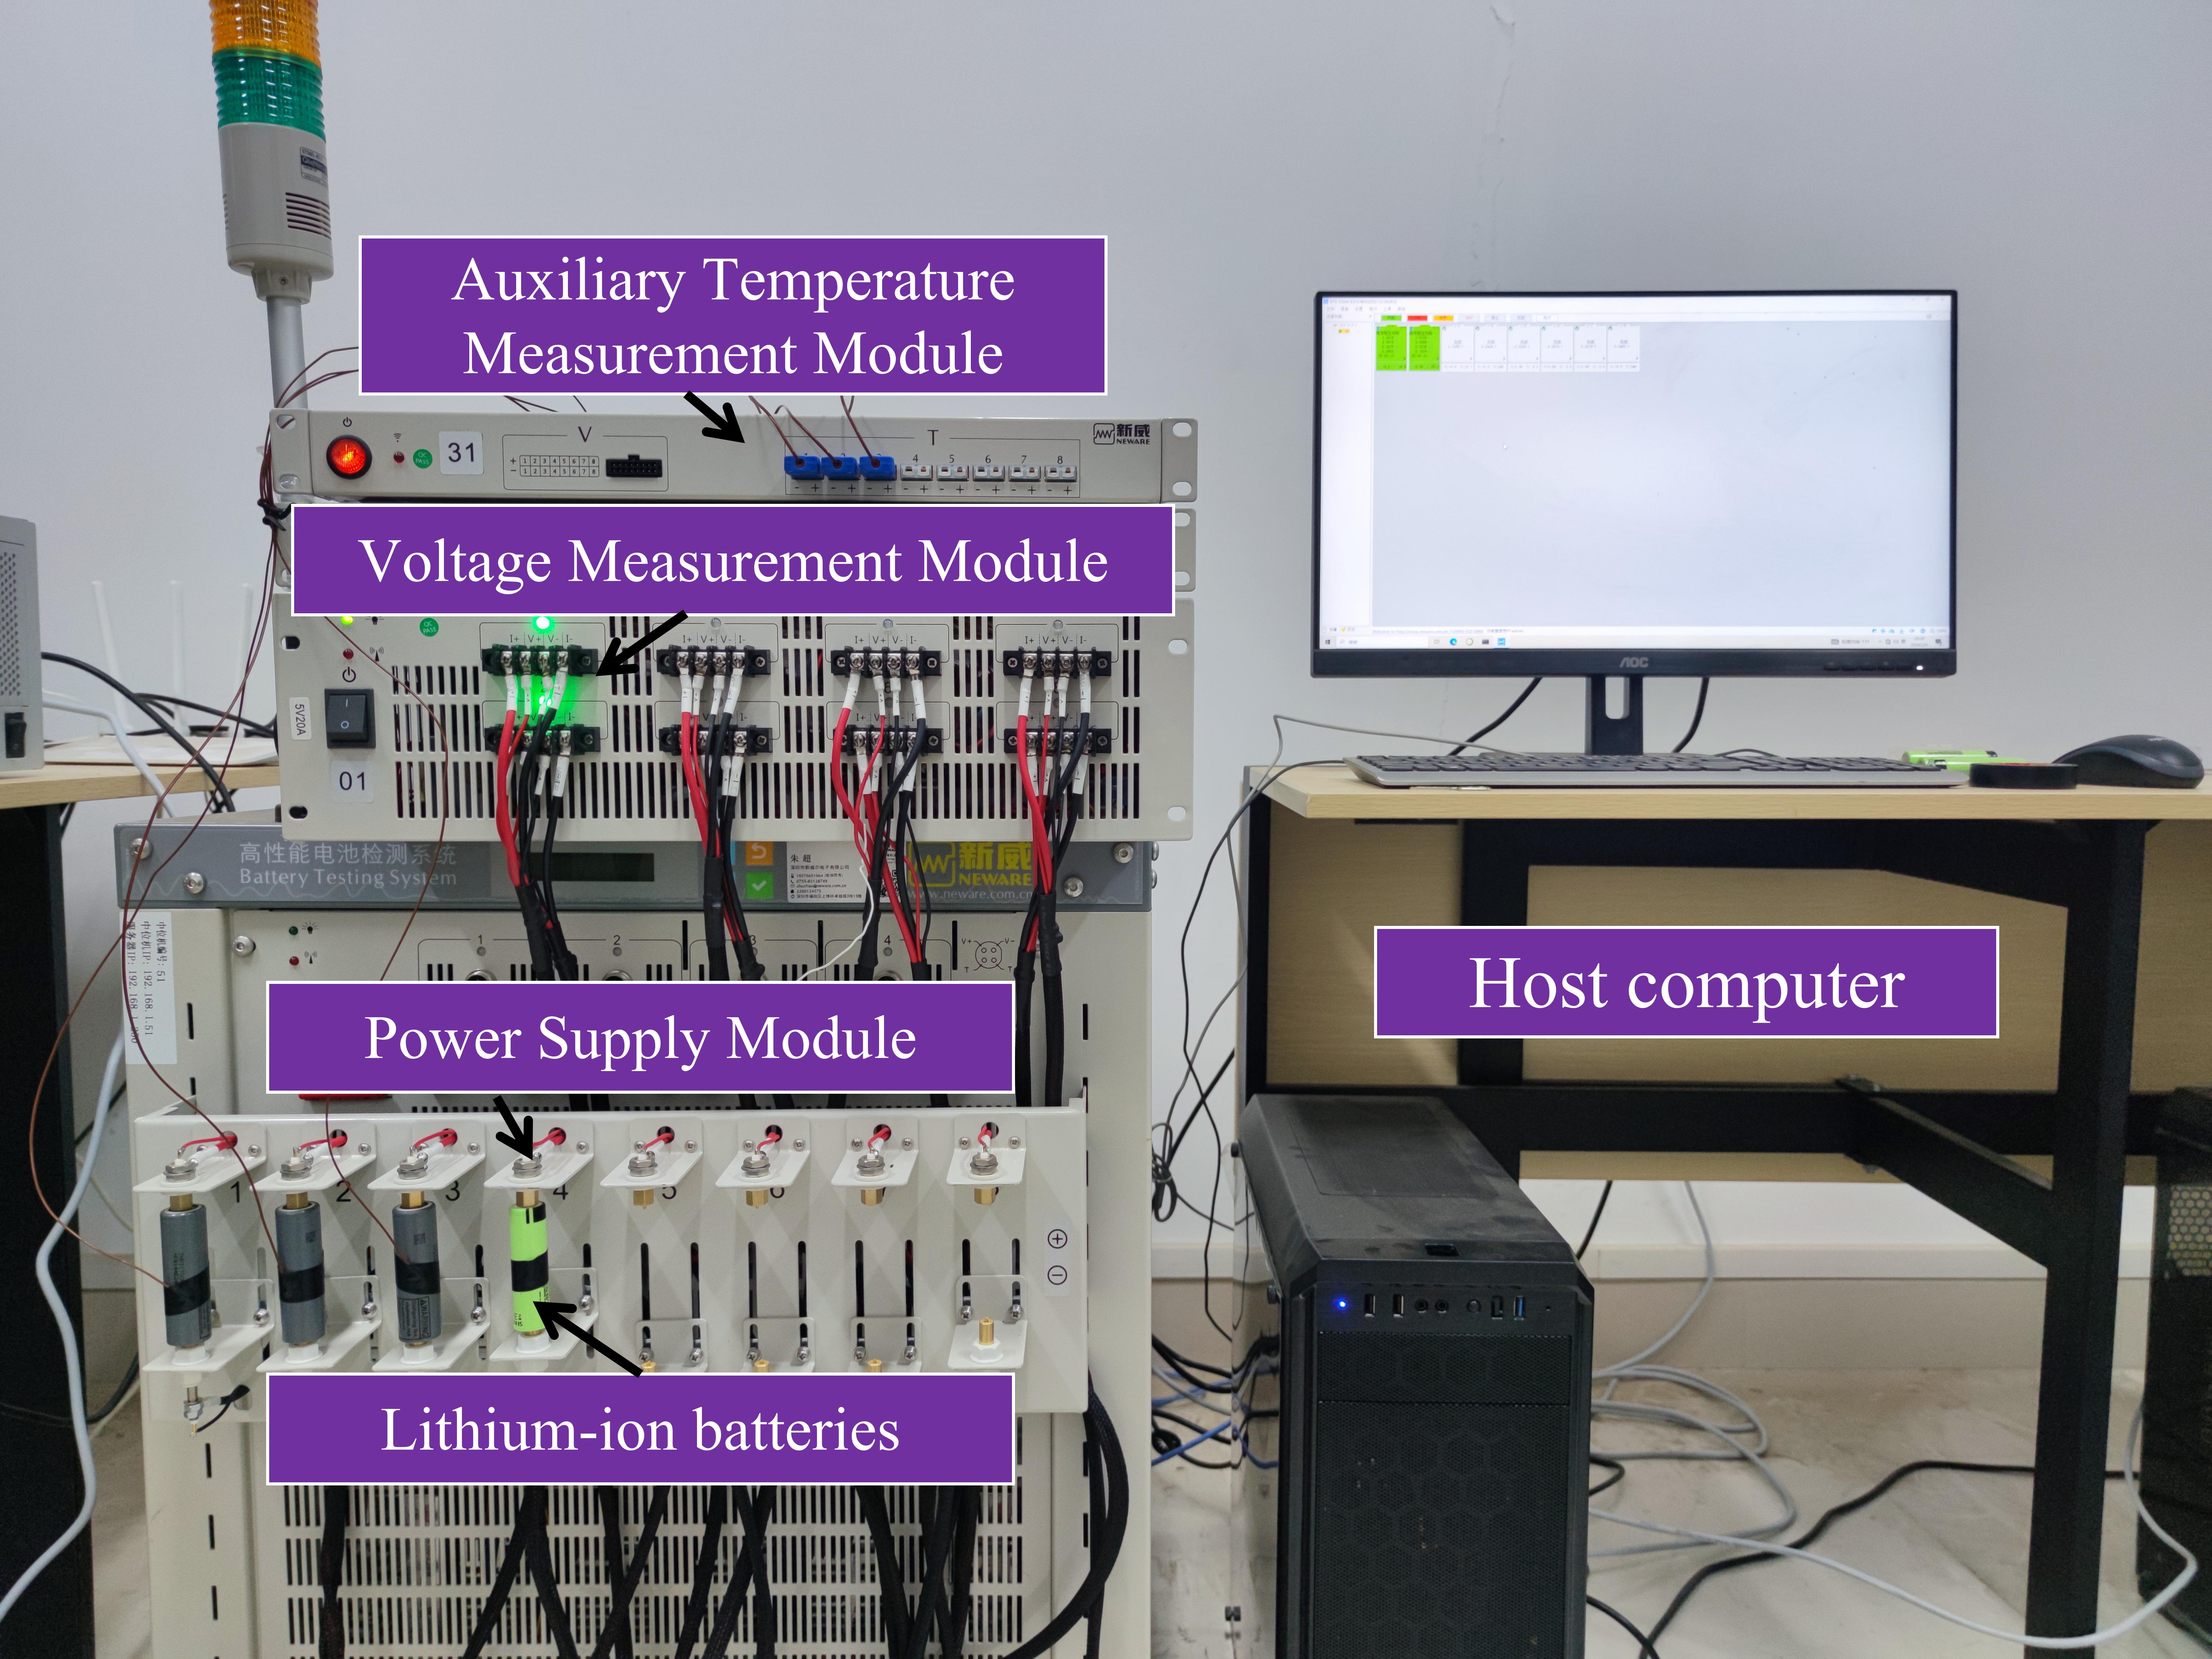
\includegraphics[width=\linewidth]{experimental_platform.png}
  \caption{Experimental Platform.}
  \label{fig:experimental_platform}
\end{figure}



\subsection{Experimental Setup}

Real-cell charging experiments were conducted using a NEWARE
CT-4008-5V20A-A battery testing system and LG INR21700 M50T
lithium-ion cells with a nominal capacity of 5 Ah. The ambient
temperature was approximately 25$^\circ$C. The experimental
platform is shown in Fig.~\ref{fig:experimental_platform}.
The battery cycler recorded the terminal voltage, current,
and charged capacity, while an auxiliary temperature module
measured the cell surface temperature.

Three charging protocols were considered: LLMBO-MO, ParEGO,
and conventional CC-CV. LLMBO-MO employed a three-stage
constant-current protocol with currents of 3.90, 3.76, and
3.00 A, switching at 40\% and 70\% SOC. ParEGO used currents
of 3.40, 4.79, and 2.99 A, switching at 11.5\% and 41.2\%
SOC. The CC-CV setting used a constant current of 1.455 A,
a constant voltage of 4.20 V, and a cutoff current of
0.05 A. All protocols were terminated after delivering
4.0 Ah, corresponding to 80\% of the nominal capacity.

For the reported three-cell comparison, each protocol was
tested twice on each cell, with discharge and rest steps
between charging runs. The results are presented as the mean
and sample standard deviation of six measurements. Charging
time, peak temperature rise, and maximum terminal voltage
were recorded. Peak temperature rise was calculated relative
to the cell surface temperature at the beginning of charging.

\begin{table}[!t]
\caption{Real-Cell Charging Results}
\label{tab:realcell_results}
\centering
\footnotesize
\setlength{\tabcolsep}{3pt}
\begin{tabular}{lccc}
\toprule
Protocol & $t_c$ (min) & $T_p$ (K) & Max. voltage (V) \\
\midrule
CC-CV &
$165.06\pm0.16$ &
$1.80\pm1.23$ &
$4.121\pm0.003$ \\
ParEGO &
$67.78\pm0.03$ &
$7.33\pm0.64$ &
$4.158\pm0.005$ \\
LLMBO-MO &
$\mathbf{64.77\pm0.01}$ &
$\mathbf{6.84\pm0.78}$ &
$4.159\pm0.006$ \\
\bottomrule
\end{tabular}
\end{table}

\subsection{Results}

The experimental results are summarized in
Table~\ref{tab:realcell_results}. LLMBO-MO achieved an
average charging time of 64.77 min, compared with
67.78 min for ParEGO, representing a 4.4\% reduction.
The average peak temperature rise was also reduced
from 7.33 K to 6.84 K. The three cells included in
the analysis exhibited the same ordering in both
charging time and peak temperature rise.

In simulation, the selected LLMBO-MO protocol strictly
Pareto-dominated the corresponding ParEGO protocol,
achieving lower charging time, peak temperature rise,
and aging indicator. The real-cell measurements confirmed
the same ordering in the two experimentally evaluated
objectives, charging time and peak temperature rise.

The conventional CC-CV setting required 165.06 min
and produced a peak temperature rise of 1.80 K,
reflecting the charging-time and thermal trade-off
associated with its lower charging current. Since
charging was terminated at 4.0 Ah, the CC-CV tests
ended before reaching the constant-voltage stage.
% END: sections/realcell.tex


\section{Conclusion}
\label{sec:conclusion}

This paper proposed LLMBO-MO, an LLM-informed multiobjective
Bayesian optimization framework for multistage battery
fast-charging protocol design under limited simulation budgets.
First, an LLM-informed warm start incorporates battery-domain
knowledge and operating constraints to generate initial charging
protocols, followed by feasibility screening and diversity-aware
selection. Second, the LLM identifies promising search regions
according to the current multiobjective preference. Third,
GP posterior cross-covariance is used to incorporate regional
guidance into the acquisition function, directing the subsequent
optimization process.

Under a budget of 56 battery-model evaluations, LLMBO-MO
achieved the highest final mean HV among the compared methods
on both battery parameterizations. On Chen2020, the mean final
HV increased from \ChenParEGOMean\ for ParEGO to
\ChenLLMBOMean, representing a \ChenFinalGain\ improvement.
On Ecker2015, the corresponding values increased from
\EckerParEGOMean\ to \EckerLLMBOMean.
The initialization and ablation studies showed that
battery-domain-informed initialization contributed substantially
to the performance improvement, while regional guidance
provided further gains.

Real-cell experiments further evaluated the optimized charging
protocols. For the three cells included in the analysis,
LLMBO-MO reduced the average charging time by 4.4\% compared
with ParEGO, from 67.78 to 64.77 min, while reducing the
average peak temperature rise from 7.33 to 6.84 K.
The selected LLMBO-MO protocol strictly Pareto-dominated
the ParEGO protocol in simulation across charging time,
peak temperature rise, and aging indicator. The real-cell
measurements showed the same performance ordering in
charging time and peak temperature rise.
Future work will investigate long-term cycling degradation
and extend the framework to different battery chemistries
and operating conditions.
% END: sections/conclusion.tex
% BEGIN: sections/references.tex
% Bibliography supplied by the authors; stable keys retained.
% Entries reordered by first citation; LGBO proceedings link verified.
% Six TTE entries replaced with topic-aligned TII articles on 2026-10-17.
% DOI and publication metadata verified against Crossref publisher records;
% original citation keys retained to preserve numbering and cross-references.

% Let references flow naturally; fixed reference breaks can create an extra page.
\begin{thebibliography}{99}

\bibitem{refFastChargeReview}
A.~Tomaszewska \textit{et al.},
``Lithium-ion battery fast charging: A review,''
\textit{eTransportation}, vol.~1, Art.~no.~100011, 2019,
\href{https://doi.org/10.1016/j.etran.2019.100011}
{doi:10.1016/j.etran.2019.100011}.

\bibitem{refTuXFC}
Y.~Gao \textit{et al.},
``Health-aware multiobjective optimal charging strategy with coupled
electrochemical-thermal-aging model for lithium-ion battery,''
\textit{IEEE Trans. Ind. Informat.},
vol.~16, no.~5, pp.~3417--3429, 2020,
\href{https://doi.org/10.1109/TII.2019.2935326}
{doi:10.1109/TII.2019.2935326}.

\bibitem{nref2}
K.~Liu, C.~Zou, K.~Li, and T.~Wik,
``Charging pattern optimization for lithium-ion batteries with an
electrothermal-aging model,''
\textit{IEEE Trans. Ind. Informat.},
vol.~14, no.~12, pp.~5463--5474, 2018,
\href{https://doi.org/10.1109/TII.2018.2866493}
{doi:10.1109/TII.2018.2866493}.

\bibitem{refFanReview}
Q.~Ouyang, J.~Chen, J.~Zheng, and H.~Fang,
``Optimal multiobjective charging for lithium-ion battery packs:
A hierarchical control approach,''
\textit{IEEE Trans. Ind. Informat.},
vol.~14, no.~9, pp.~4243--4253, 2018,
\href{https://doi.org/10.1109/TII.2018.2825245}
{doi:10.1109/TII.2018.2825245}.

\bibitem{refHuMulti}
N.~Tian, H.~Fang, and Y.~Wang,
``Real-time optimal lithium-ion battery charging based on explicit
model predictive control,''
\textit{IEEE Trans. Ind. Informat.},
vol.~17, no.~2, pp.~1318--1330, 2021,
\href{https://doi.org/10.1109/TII.2020.2983176}
{doi:10.1109/TII.2020.2983176}.

\bibitem{refGPA}
B.-C.~Wang, Y.-Y.~Mao, Y.~Wang, and H.-X.~Li,
``Gaussian process-accelerated multiobjective evolutionary design
of charging process considering multiple user preferences,''
\textit{IEEE Trans. Ind. Informat.},
vol.~20, no.~8, pp.~10123--10133, 2024,
\href{https://doi.org/10.1109/TII.2024.3388602}
{doi:10.1109/TII.2024.3388602}.

\bibitem{nref3}
P.~M.~Attia \textit{et al.},
``Closed-loop optimization of fast-charging protocols for batteries
with machine learning,''
\textit{Nature}, vol.~578, pp.~397--402, 2020,
\href{https://doi.org/10.1038/s41586-020-1994-5}
{doi:10.1038/s41586-020-1994-5}.

\bibitem{nref7}
B.~Jiang \textit{et al.},
``Fast charging design for lithium-ion batteries via Bayesian
optimization,''
\textit{Appl. Energy}, vol.~307, Art.~no.~118244, 2022,
\href{https://doi.org/10.1016/j.apenergy.2021.118244}
{doi:10.1016/j.apenergy.2021.118244}.

\bibitem{nref8}
X.~Wang and B.~Jiang,
``Multi-objective optimization for fast charging design of lithium-ion
batteries using constrained Bayesian optimization,''
\textit{J. Power Sources}, vol.~584, Art.~no.~233602, 2023,
\href{https://doi.org/10.1016/j.jpowsour.2023.233602}
{doi:10.1016/j.jpowsour.2023.233602}.

\bibitem{nref6}
B.~Shahriari \textit{et al.},
``Taking the human out of the loop: A review of Bayesian optimization,''
\textit{Proc. IEEE}, vol.~104, no.~1, pp.~148--175, 2016,
\href{https://doi.org/10.1109/JPROC.2015.2494218}
{doi:10.1109/JPROC.2015.2494218}.

\bibitem{refDongBO}
G.~Dong, Z.~Zhu, Y.~Lou, J.~Yu, L.~Wu, and J.~Wei,
``Optimal charging of lithium-ion battery using distributionally robust
model predictive control with Wasserstein metric,''
\textit{IEEE Trans. Ind. Informat.},
vol.~20, no.~5, pp.~7630--7640, 2024,
\href{https://doi.org/10.1109/TII.2024.3363079}
{doi:10.1109/TII.2024.3363079}.

\bibitem{refZhuMOBO}
Y.~Hao, Q.~Lu, X.~Wang, and B.~Jiang,
``Adaptive model-based reinforcement learning for fast-charging
optimization of lithium-ion batteries,''
\textit{IEEE Trans. Ind. Informat.},
vol.~20, no.~1, pp.~127--137, 2024,
\href{https://doi.org/10.1109/TII.2023.3257299}
{doi:10.1109/TII.2023.3257299}.

\bibitem{refEIMO}
B.-C.~Wang, Y.-Y.~Mao, J.-M.~Jia, J.~Liu, and Y.~Wang,
``Experience-informed multiobjective optimization for fast
charging design of lithium-ion batteries,''
\textit{IEEE Trans. Autom. Sci. Eng.},
vol.~23, pp.~16843--16856, 2026,
\href{https://doi.org/10.1109/TASE.2026.3716925}
{doi:10.1109/TASE.2026.3716925}.

\bibitem{refPriorCharging}
W.~Jeong, S.~Heo, and J.~H.~Lee,
``Health-conscious charging of lithium-ion batteries using
Bayesian optimization guided by a semi-empirical aging model,''
\textit{J. Energy Storage},
vol.~141, Art.~no.~119348, 2026,
\href{https://doi.org/10.1016/j.est.2025.119348}
{doi:10.1016/j.est.2025.119348}.

% Newly added: Prior-informed Bayesian optimization
\bibitem{refPiBO}
C.~Hvarfner, D.~Stoll, A.~Souza, M.~Lindauer,
F.~Hutter, and L.~Nardi,
``$\pi$BO: Augmenting acquisition functions with user beliefs
for Bayesian optimization,''
in \textit{Proc. Int. Conf. Learn. Represent. (ICLR)}, 2022.
[Online]. Available:
\url{https://arxiv.org/abs/2204.11051}.

\bibitem{nref12}
T.~Liu, N.~Astorga, N.~Seedat, and M.~van der Schaar,
``Large language models to enhance Bayesian optimization,''
in \textit{Proc. Int. Conf. Learn. Represent. (ICLR)}, 2024.
[Online]. Available:
\url{https://openreview.net/forum?id=OOxotBmGol}.

% Newly added: LLM-guided Bayesian optimization
\bibitem{refBORA}
A.~Ciss\'e, X.~Evangelopoulos, V.~V.~Gusev,
and A.~I.~Cooper,
``Language-based Bayesian optimization research assistant (BORA),''
in \textit{Proc. 34th Int. Joint Conf. Artif. Intell. (IJCAI)},
2025, pp.~4967--4975,
\href{https://doi.org/10.24963/ijcai.2025/553}
{doi:10.24963/ijcai.2025/553}.

\bibitem{refBianLLM}
L.~Hou, Y.~Shang, T.~Qiu, X.~Zhang, Y.~Zhu, and X.~Gu,
``Prompt-driven fine-tuning large language model for multistate
coestimation of lithium-ion batteries,''
\textit{IEEE Trans. Ind. Informat.},
vol.~22, no.~8, pp.~6647--6658, 2026,
\href{https://doi.org/10.1109/TII.2025.3631017}
{doi:10.1109/TII.2025.3631017}.

\bibitem{refKuaiLLMBO}
X.~Kuai, J.-H.~Ren, B.-C.~Wang, and Y.~Feng,
``Large language model-enhanced Bayesian optimization for
parameter identification of lithium-ion batteries,''
\textit{J. Energy Storage},
vol.~135, Art.~no.~118198, 2025,
\href{https://doi.org/10.1016/j.est.2025.118198}
{doi:10.1016/j.est.2025.118198}.

\bibitem{ref5}
X.~Yuan, Z.~Chen, J.~Zhang, H.~Xiong,
N.~Ye, Y.~Li, and Q.~Gu,
``Unleashing LLMs in Bayesian optimization:
Preference-guided framework for scientific discovery,''
in \textit{Proc. Int. Conf. Learn. Represent. (ICLR)}, 2026.
[Online]. Available:
\url{https://proceedings.iclr.cc/paper_files/paper/2026/hash/85381f4549b5ddf1d48e2e287d7d3d15-Abstract-Conference.html}.

\bibitem{refSPMe}
S.~J.~Moura, F.~B.~Argomedo, R.~Klein,
A.~Mirtabatabaei, and M.~Krstic,
``Battery state estimation for a single particle model
with electrolyte dynamics,''
\textit{IEEE Trans. Control Syst. Technol.},
vol.~25, no.~2, pp.~453--468, 2017.

\bibitem{refAgingModel}
G.~Suri and S.~Onori,
``A control-oriented cycle-life model for hybrid electric
vehicle lithium-ion batteries,''
\textit{Energy}, vol.~96, pp.~644--653, 2016.

\bibitem{ref4}
J.~Knowles,
``ParEGO: A hybrid algorithm with on-line landscape approximation
for expensive multiobjective optimization problems,''
\textit{IEEE Trans. Evol. Comput.},
vol.~10, no.~1, pp.~50--66, 2006.

\bibitem{ref8}
C.-H.~Chen, F.~Brosa Planella, K.~O'Regan, D.~Gastol,
W.~D.~Widanage, and E.~Kendrick,
``Development of experimental techniques for parameterization
of multi-scale lithium-ion battery models,''
\textit{J. Electrochem. Soc.},
vol.~167, no.~8, Art.~no.~080534, 2020.

\bibitem{ref9}
M.~Ecker, T.~K.~D.~Tran, P.~Dechent,
S.~K\"abitz, A.~Warnecke, and D.~U.~Sauer,
``Parameterization of a physico-chemical model of a lithium-ion
battery: I. Determination of parameters,''
\textit{J. Electrochem. Soc.},
vol.~162, no.~9, pp.~A1836--A1848, 2015.

\bibitem{refDISK}
Z.~Zhang, Y.~Wang, G.~Sun, and T.~Pang,
``A distribution information-based Kriging-assisted evolutionary
algorithm for expensive many-objective optimization problems,''
\textit{IEEE Trans. Evol. Comput.},
vol.~29, no.~6, pp.~2656--2670, 2025.

\bibitem{refPIMD}
Y.~Li, W.~Li, S.~Li, and Y.~Zhao,
``An infill sampling criterion based on improvement of probability
and mapping crowding distance for expensive multi/many-objective
optimization,''
\textit{Eng. Appl. Artif. Intell.},
vol.~133, Art.~no.~108616, 2024.

\bibitem{refNSGAII}
K.~Deb, A.~Pratap, S.~Agarwal, and T.~Meyarivan,
``A fast and elitist multiobjective genetic algorithm: NSGA-II,''
\textit{IEEE Trans. Evol. Comput.},
vol.~6, no.~2, pp.~182--197, 2002,
\href{https://doi.org/10.1109/4235.996017}
{doi:10.1109/4235.996017}.

\end{thebibliography}
% END: sections/references.tex

\end{document}
